\documentclass{modelica}

\addbibresource{paper.bib}

\hypersetup{%
  pdftitle  = {Real-time Simulation and CHiL Testing of Power System Stabilizers on Microcontrollers with Modelica and eFMI},
  pdfauthor = {Luigi Vanfretti, Christoff Bürger, Joseph Pizzimenti, Kyle Wilt, Hao Chang},
  pdfsubject = {American Modelica and FMI Conference 2026},
  pdfkeywords = {power systems, power grid, power system stabilizer, real-time simulation, CHiL, embedded control, Modelica, eFMI, Dymola, STM32, ARM Cortex-M},
  colorlinks,
  linkcolor=black,
  urlcolor=black,
  citecolor=black,
  pdfpagelayout = SinglePage,
  pdfcreator = pdflatex,
  pdfproducer = pdflatex}

% User packages
\usepackage[inkscapelatex=false]{svg}
\usepackage{booktabs}
\usepackage{amsmath}

\usepackage[dvipsnames]{xcolor}
\definecolor{mygreen}{HTML}{008c48}
\definecolor{myblue}{HTML}{1c6cc8}
\definecolor{mygray}{HTML}{999999}

\usepackage{listings}
\input{./listings-modelica.cfg}
\lstset{%
    language=modelica,
    basicstyle=\fontsize{7.5pt}{9pt}\ttfamily,
    commentstyle=\color{mygreen}\itshape,
    keywordstyle=[1]\color{myblue}\bfseries,
    keywordstyle=[2]\color{myblue}\bfseries,
    keywordstyle=[3]\color{myblue}\bfseries,
    xleftmargin=2.5ex,
    numbersep=2.5pt}

\usepackage{siunitx}
\sisetup{per-mode = symbol}

% Begin the document
\begin{document}
\thispagestyle{empty}

\title{Real-time Simulation and CHiL Testing of Power System Stabilizers on Microcontrollers with Modelica and eFMI}
\author[1]{Luigi Vanfretti}
\author[2]{Christoff Bürger}
\author[1]{Joseph Pizzimenti}
\author[1]{Kyle Wilt}
\author[1]{Hao Chang}
\affil[1]{Electrical, Computer and Systems Engineering Department, Rensselaer Polytechnic Institute, USA, {\small\texttt{\{vanfrl,pizzij,wiltk2,changh7\}@rpi.edu}}}
\affil[2]{Dassault Systèmes AB, Lund, Sweden, {\small\texttt{christoff.buerger@3ds.com}}}

\maketitle\thispagestyle{empty} %% <-- you need this for the first page

% User definitions
\newcommand{\myitemsep}{\itemsep-0.1em}
\newcommand{\regtm}{\textsuperscript{\textregistered}}
\newcommand{\controller}{\textcolor{mygreen}{\textbf{\underline{controller}}}}
\newcommand{\plant}{\textcolor{myblue}{\textbf{\underline{plant}}}}
\newcommand{\generatorunit}{\textcolor{mygray}{\textbf{\underline{generator unit}}}}
\newcommand{\squishlist}{
 \begin{list}{$\bullet$}
  { \setlength{\itemsep}{0pt}
     \setlength{\parsep}{3pt}
     \setlength{\topsep}{3pt}
     \setlength{\partopsep}{0pt}
     \setlength{\leftmargin}{1.5em}
     \setlength{\labelwidth}{1em}
     \setlength{\labelsep}{0.5em} } }
\newcommand{\squishlisttwo}{
 \begin{list}{$\bullet$}
  { \setlength{\itemsep}{0pt}
    \setlength{\parsep}{0pt}
    \setlength{	opsep}{0pt}
    \setlength{\partopsep}{0pt}
    \setlength{\leftmargin}{2em}
    \setlength{\labelwidth}{1.5em}
    \setlength{\labelsep}{0.5em} } }
\newcommand{\squishend}{
  \end{list}  }

% Actual paper contents
\begin{abstract}
Modern power grids face significant stability challenges, as shown by recent incidents such as the 2025 oscillations of the Iberian grid. These issues highlight the need for robust Model-Based Systems Engineering (MBSE) to enable rapid control redesign and deployment. Yet, the move to Controller Hardware-in-the-Loop (CHiL) testing is hindered by inefficient, manual re-implementation workflows, complex tooling and technology stacks with high software and hardware costs, and challenges to incorporate real-time suited plant models for controller testing. This lack of efficiency disrupts the traceability between design and implementation.

This paper pioneers an automated workflow using the Modelica language and the eFMI (Functional Mock-up Interface for embedded systems) standards to bridge this gap. We introduce the \texttt{OpenIPSL\_CHIL} library, which provides extensions to the Open-Instance Power System Library (OpenIPSL) specifically for embedded real-time applications. Using Dymola's eFMI tooling, both the power system stabilizer (PSS) (a damping controller) and the generator interconnected to a power grid (the plant) are systematically synthesized into production-ready code and deployed onto low-cost ARM-based microcontrollers of the STM32 ecosystem.

The methodology is validated by a full suite of Model-in-the-Loop (MiL), Software-in-the-Loop (SiL), and CHiL tests, ensuring that embedded behavior aligns with physics-based offline simulations, with the non-functional quality of generated production code ensured in the process by MISRA C:2023 and SEI CERT C Coding Standard compliance and real-time capability checks.

The developed framework offers an open-source, traceable, and cost-effective alternative to expensive proprietary real-time platforms and significantly reduces capital expenditures for grid control research.
\end{abstract}

\noindent\emph{Keywords: power systems, power grid, power system stabilizer, real-time simulation, CHiL, embedded control, Modelica, eFMI, Dymola, STM32, ARM Cortex-M}

\section{Introduction}

\subsection{Motivation}

\paragraph{Challenges of power grid stability require better power system control:} Modern power grids need a robust Model-Based Systems Engineering (MBSE) method to connect control design with real-world control deployment and routine tuning. Recent incidents, including the inter-area oscillations observed in Europe in 2016 and 2017 \cite{ENTSOE_2016, ENTSOE_2017}, highlight how crucial proper tuning of a Power System Stabilizer (PSS) is to preserve adequate damping throughout the system. More recently, the Iberian grid incident of 2025 \cite{ENTSOE_Iberian_Factual_2025, ENTSOE_Iberian_2026} revealed complex 0.63 Hz and 0.2 Hz oscillations. Although initiated by inverter-based resources, the incident report emphasizes that poor coordination and the absence of detailed models for active damping controls—including existing PSS—limited operators’ ability to foresee and contain the disturbance, forcing rapid revisions to operating rules.

Discrepancies between simulations and field behavior often stem from outdated modeling workflows that fail to capture actual hardware logic. Such control-induced issues have been increasingly observed in inverter-based resources, including irregular dynamics in wind plants due to setpoint truncation \cite{Pudasaini2026} and non-sinusoidal responses in solar PV installations \cite{Mishra2026}. This fragility extends to traditional synchronous generation; for example, a 1.5 Hz forced oscillation event was recently triggered during a reactive power capability test at a conventional power plant in Dominion \cite{Mishra2024_Greensville}. Although the power plant model was accurate, the PSS was not designed for the specific operating condition encountered, leading to sustained oscillations. These challenges demand adaptable controllers that can be redesigned and deployed throughout their operational lifecycle \cite{Bombois2024, Lauria2024_SEGAN}.

\paragraph{Development and deployment challenges of power system controllers hinder adoption of novel stabilizers:} When developing new control strategies to address grid stability issues, the path from new control designs to Controller Hardware-in-the-Loop (CHiL) tests is currently inefficient due to a lack of dynamic model portability and broken traceability. Offline power system simulation tools, such as PSS\regtm{}E or PSCAD\regtm{}, cannot be directly used for real-time simulation. This necessitates manual re-implementation, which creates ambiguity and consumes significant time and resources. Furthermore, control code is often hardware-dependent; for example, specialized wide-area PSS implementations frequently require bespoke code for specific platforms such as National Instruments\regtm{} hardware \cite{Rebello2020}. This fragmented workflow and the high cost of real-time simulators and prototyping hardware, such as CompactRIO\regtm{} (National Instruments), create significant barriers to deploying novel control strategies.

\paragraph{eFMI tooling for Modelica provides new opportunities for power system design and control:} The acausal, equation-based Modelica\regtm{}\footnote{\label{fnt:modelica}\tiny{\url{https://modelica.org/language/}}} modeling language has been successfully used to design and simulate power systems and grids~\cite{ipsl,openipsl}. Its object-oriented, system-level design is particularly well-suited for rapid prototyping of design variants and modifications~\cite{Burger2019}. Modelica also provides the means of modeling clocked subsystems, such as digital controllers, seamlessly integrated within the continuous simulation of plant models \cite{Elmqvist2012}. This makes Modelica an excellent choice for physics-based modeling and simulation of power systems with novel stabilizing controllers. Recent support for the new eFMI\regtm{} Standard\footnote{\label{fnt:efmi-website}\tiny{\url{https://www.efmi-standard.org/}}} \cite{eFMI_Standard} by Modelica tools (such as Dymola\regtm{}\footnote{\label{fnt:dymola}\tiny{\url{https://www.3ds.com/products/catia/dymola}}}) extends the applicability of physics models beyond offline simulation to the embedded domain. The eFMI capabilities provided by Dymola facilitate the deployment of Modelica-based models in safety-critical applications that operate under stringent hard real-time constraints.
\subsection{Contributions}

This paper pioneers a Modelica and eFMI-based approach to design power system damping controllers. We use Modelica and eFMI to (1) rapidly prototype and conduct Model- and Software-in-the-Loop (MiL, SiL) testing of PSS designs, (2) deploy the designed models (plant and controller models) directly onto microcontrollers, and finally (3) verify in CHiL tests that embedded behavior aligns with the offline simulations. Our approach solves many of the previously bespoke design, development, and deployment challenges associated with a PSS:

\squishlist
    \item Common physics-based models are the single source of truth, reducing model-misalignment and inconsistency errors, and preventing behavior that violates or neglects laws of physics.
    \item The MBSE approach reduces errors during the transition from physics-based models to actual embedded solutions, as is typical for manually developed control code or code based on heterogeneous tooling at different abstraction levels that requires manual adaptation within deep technology stacks.
    \item Directly deploying models (controller and plant) on microcontrollers enables rapid control prototyping and reduces the risk of late detection of system-integration issues. Expensive real-time platforms can be avoided and the complexity of the tooling stacks involved can be reduced.
    \item Gaps in model portability and traceability are minimized.
\squishend

\noindent{}To validate our approach, we designed real-time-suited Modelica models based on the Open-Instance Power System Library\footnote{\label{fnt:openipsl}\tiny{\url{https://github.com/OpenIPSL/OpenIPSL}}} (\texttt{OpenIPSL}), generated the corresponding eFMI solutions in Dymola, system-integrated them on STM32\regtm{} microcontrollers with the help of STM32CubeMX\footnote{\label{fnt:stm32cubemx}\tiny{\url{https://www.st.com/en/development-tools/stm32cubemx.html}}} and STM32CubeIDE\footnote{\label{fnt:stm32cubeide}\tiny{\url{https://www.st.com/en/development-tools/stm32cubeide.html}}}, and systematically validated each step in respective MiL, SiL, and CHiL tests. All materials are provided open-source under the 3-Clause BSD License, as an extensible workbench framework\footnote{\label{fnt:pss-repository}\tiny{\url{https://github.com/ALSETLab/efmi-pss-use-case}}} ultimately empowering researchers to rapidly prototype grid controllers with guaranteed traceability and significantly reduced capital expenditure. Our approach provides a low-cost proof-of-concept platform for PSS microcontroller prototyping.

\subsection{Paper structure}

The remainder of this paper is organized as follows: Section \ref{sec:efmi-and-use-case-workflow-overview} provides an overview of the eFMI Standard and the proposed MBSE workflow. Section \ref{sec:modeling-for-mil-testing} details the modeling approach and MiL validation using the new \texttt{OpenIPSL\_CHIL} library. Section \ref{sec:efmuGenAndSiL} discusses the synthesis of eFMUs and SiL tests and code analyses for such, while Section \ref{sec:STM32-integration-of-eFMUs} describes the system integration on STM32 hardware. Real-time simulation results and CHiL performance analyses are presented in Section \ref{sec:rtchil}. Section \ref{sec:conclu} provides conclusions and outlines future work, followed by an Appendix summarizing the related work that highlights the limitations of current practices in the power industry related to damping controls.

\section{eFMI \& use-case workflow overview}\label{sec:efmi-and-use-case-workflow-overview}

This section provides a high-level overview of the eFMI Standard insofar as it is required to identify the main artifacts and generative model-based software engineering (MBSE) processes that it provides for our use-case; afterward, the objectives and workflow of the actual tooling we are using are presented.

\subsection{The eFMI Standard}\label{sec:efmi-standard}

The eFMI Standard\footref{fnt:efmi-website} \cite{eFMI_Standard} is an open standard of the Modelica Association\regtm{}\footnote{\tiny{\url{https://modelica.org/association/}}}. The official website\footref{fnt:efmi-website} provides a concise summary of the primary objectives of eFMI:
\blockquote{The \textit{eFMI\regtm{} Standard} is an open standard for the stepwise, model-transformation-based development of advanced control functions suited for safety-critical and real time targets. Its container architecture defines the common ground for collaboration among the stake-holders and toolchains along the various abstraction levels from high-level modeling and simulation -- e.g., a-causal, equation-based physics in Modelica -- down to actual embedded code. The model representations it defines are interlinked for traceability and semi-automatic code generation and do not only capture functional, but also non-functional quality requirements like coding standards, static memory allocation, worst time execution, and documentation, enabling credible development within a standardized workspace.\footnote{Originally written by Christoff Bürger.}}

\noindent{}The abstraction levels eFMI supports---each represented by a dedicated container type with well-defined content and with all containers of an embedded solution wrapped in a single embedded functional mock-up unit (eFMU)---are\footnote{Parts of the following Algorithm Code container section are from \cite{Kamp2025} and have been originally written by Christoff Bürger.} (note that, in contrast to FMUs, an eFMU is an open workspace container potentially still in development; eFMI can be used as a credible MBSE process to develop---i.e., implement---co-simulation FMUs for safety-critical real-time simulation):

\paragraph{Algorithm Code container:} Algorithmic high-level solution of a sampled system. Algorithms are implemented in GALEC, a new \underline{\textbf{g}}uarded \underline{\textbf{a}}lgorithmic \underline{\textbf{l}}anguage for \underline{\textbf{e}}mbedded \underline{\textbf{c}}ontrol defined in the eFMI Standard. Although imperative, GALEC provides many high-level concepts like multi-dimensional arithmetic operators, derived but well-defined dimensional sizes, and a built-in function standard library to abstract target-specific characteristics and provide common math operations, including interpolation and solving systems of linear equations. GALEC is computationally safe; a powerful static evaluation concept is used to guarantee all indexing is within bounds, all loops have an upper-bound, and all potential runtime errors like IEEE 754 not-a-number (NaN) values, singular linear equation systems or domain errors of built-in functions (like poles of trigonometric functions) are handled or explicitly exposed to the runtime environment (error signals of interface functions). GALEC is also well-defined regarding its imperative side-effects; for every two GALEC statements it is decidable whether they can be swapped, enabling, together with its well-defined dimensionality analysis, target-specific concurrent execution optimizations. Note that GALEC has no foreign function interface (FFI), only built-in functions; GALEC programs are therefore by nature self-contained. From a Modelica perspective, for example, a GALEC solution of a sampled system of equations (potentially with events or mixed system of equations) requires the solver to be inline-integrated as GALEC code, eliminating dependencies on third party numerical libraries.

These characteristics---self-contained, target independent, high abstraction level, and well-defined behavior under all circumstances---make GALEC an ideal intermediate language between simulation tools (that can target GALEC for code generation) and the embedded domain (where GALEC can serve as a source for code generation). Once a simulation tool finds a sampled solution for the simulation problem---which is not always possible for general equation systems---and expresses it as GALEC program, further tooling towards embedded C code "only" has to preserve these characteristics and can focus on code optimization (e.g., loop and multi-dimensional expression unrolling, or concurrent execution) and embedded target environment compliance (e.g., compliance with style guidelines, code analysers, interfaces, or other system integration requirements).

The sampled block-interface of the GALEC program of an Algorithm Code container is also exposed by the XML manifest file of the container, such that derived eFMU artifacts, like production code, can refer to it; this is important for traceability, but also to enable tooling to work with eFMUs without having to process GALEC (e.g., if just using production code without generating it). Naturally, each eFMU must have a single Algorithm Code container.

\paragraph{Production Code containers:} Target-specific production code (C program) implementing the GALEC program of the eFMU's Algorithm Code container. Typical challenges of production code generators are related to efficiently translating GALEC multi-dimensional arithmetic operations, providing implementations of the used built-in functions (or preferable reuse target ecosystem routines considering restricted availability of the C Standard Library), complying with embedded coding standards like MISRA C:2023 or the SEI CERT C Coding Standard\footnote{\label{fnt:sei-cert-c}\tiny{\url{https://cmu-sei.github.io/secure-coding-standards/sei-cert-c-coding-standard/}}}, following target ecosystem system integration APIs, generating ISO/IEC 9899 (C11, C17, C24, etc.) compliant code, and finding good trade-offs between portability and optimization.

An XML manifest file within each Production Code container maps the respective code's API to the well-defined (i.e., standardized in eFMI) block-interface of the eFMU's Algorithm Code container. This enables automatic system integration---as for example exploited by Dymola's production code export options presented in Section \ref{sec:production-code-export}---although eFMI does not standardize any production code interface (unlike FMI\footnote{\label{fnt:fmi}\tiny{\url{https://fmi-standard.org/}}} 3.0, which does with \texttt{fmi3Functions.h}). Naturally, an eFMU can contain many different production codes, e.g., for various floating-point precisions or code optimizations.

\paragraph{Binary Code containers:} Target specific binary code generated from one of the eFMU's Production Code containers. An XML manifest file lists the target platform, used compiler and linker options, and links back to the source Production Code container. Naturally, an eFMU can contain many different binaries, even for the same production code (e.g., based on different compiler and linker settings like debug and release versions, or for different targets).

\paragraph{Behavioral Model containers:} Test scenarios with reference trajectories stored in comma separated value (CSV) files and additional meta-information---like trajectory units, the index-wise splicing of multi-dimensional trajectories into separate scalar trajectories, absolute and relative tolerances, or scenario descriptions---stored in an XML manifest file. Two kinds of test scenarios are supported: variable time grid scenarios and equidistant time grid scenarios. The latter enforce a fixed sampling period within strict time tolerances between adjacent trajectory points, as, for example, typical for HiL tests. Variable time grid scenarios are more flexible, but require well-defined interpolation (and for that reason typically higher tolerances) when used for testing a sampled system like GALEC programs or derived production code; they typically stem from continuous simulations with flexible step size (e.g., DASSL).

Naturally, an eFMU can contain many Behavioral Model containers, e.g., created by different simulation or measurement tools. Automatic instantiation---although the APIs of production and binary codes are not standardized---for testing is possible thanks to all eFMU containers (including Behavioral Model ones) linking back to the well-defined block-interface of an eFMU's Algorithm Code container.

\subsection{Use-case tooling \& workflow}

In our use-case, we develop two models with the final objective of embedded deployment for CHiL testing: a power system stabilizer (i.e., an actual controller) and a hard real-time simulation of the controlled power system (i.e., the plant model). To that end, we used the following tools:

\squishlist
    \item \textbf{Dymola\regtm{}\footref{fnt:dymola} 2026x Refresh 1:} Physics-based design of Modelica models of the controller and plant; systematic MiL testing of design variants from continuous to sampled experiments with controller and plant models refined for eFMI (cf. Section \ref{sec:modeling-for-mil-testing}); controller and plant eFMU generation (cf. Section \ref{sec:eFMU-configurations}) and SiL tests of their production code against MiL experiments (cf. Section \ref{sec:modelica-based-sil-tests}).
    \item \textbf{Cppcheck\regtm{} Premium\footnote{\label{fnt:cppcheck-premium}\tiny{\url{https://www.cppcheck.com/}}} 26.3.0 and clang-tidy\footnote{\label{fnt:clang-tidy}\tiny{\url{https://clang.llvm.org/extra/clang-tidy/}}} (Clang Tools 19.1.5):} Strict code quality analyses---in particular for MISRA C:2023 compliance---of the eFMU production code of controller and plant (cf. Section \ref{sec:production-code-quality-analyses}).
    \item \textbf{STM32CubeMX\footref{fnt:stm32cubemx} 6.17.0:} Selection of STM32 microcontrollers for controller and plant; configuration of their peripherals---like pins, DACs, and timers---and generation of respective template code linking to the STM32CubeH7\footnote{\tiny{\url{https://www.st.com/en/embedded-software/stm32cubeh7.html}}} 1.13.0 software package with hardware abstraction layer (HAL), lower-layer (LL) drivers, and Arm\regtm{} Cortex\regtm{}-M Common Microcontroller Software Interface Standard (CMSIS) implementations\footnote{STM32CubeH7 also includes middleware libraries supporting, for example, a USB stack, TCP/IP networking stack, file system, or even real-time operation system (RTOS); we do not use any of the STM32CubeH7 middleware libraries.} (cf. Section \ref{sec:STM32CubeMX}).
    \item \textbf{STM32CubeIDE\footref{fnt:stm32cubeide} 2.1.0:} Import of CubeMX generated template codes of controller and plant as individual C development projects; incorporation of their eFMU Production Code containers as symbolically linked source and include directories; system integration of eFMU production codes into the \texttt{main()} execution routine of the microcontrollers; compilation and deployment on STM32 boards (cf. Section \ref{sec:STM32CubeIDE}).
    \item \textbf{WaveForms\footnote{\label{fnt:waveforms}\tiny{\url{https://digilent.com/shop/waveforms/}}} 3.25.1:} Interactive stimuli generation and plotting of CHiL test signals with a Digilent\regtm{} Analog Discovery 3 oscilloscope (cf. Section \ref{sec:rtchil}).
\squishend

\noindent{}Note, that our approach to deploy the plant model---which is required for CHiL testing the controller---directly on a microcontroller avoids the need for a real-time HiL platform, e.g., from dSPACE\regtm{}, Typhoon HIL\regtm{} or OPAL-RT Technologies\regtm{}; this reduces not only hardware costs but also the complexity of the required software and tooling stack and its licensing. All tools, except Dymola and Cppcheck Premium, are freely available. To generate eFMUs, the \textit{Dymola Source Code Generation} option, besides a standard Dymola license, is required. Although an open-source version of Cppcheck exists (and could have been used), its MISRA C:2023 and SEI CERT C Coding Standard\footref{fnt:sei-cert-c} coverage is significantly inferior to the commercial Premium version. And while production code analyses are optional for our use-case, they are of general interest for certification (Cppcheck Premium for example has TÜV SÜD\regtm{}\footnote{\tiny{\url{https://www.tuvsud.com/en}}} certification against EN 50128, EN 50657, EN 50716, IEC 61508, and ISO 26262).

\section{Modeling and MiL testing}\label{sec:modeling-for-mil-testing}

This section describes the power system model that will be used to demonstrate the application of eFMI to both synthesis and deployment of the controller code. The system to be modeled is illustrated in Figure \ref{fig:overview}, which shows a power plant interconnected to a power grid. The power plant's generator, a synchronous machine, is equipped with a PSS that is placed before the Excitation Control System (ECS). 

\begin{figure}[t!]
\centerline{\includesvg[width=0.975\columnwidth]{./figures/f01-overview-w.svg}}
    \caption{Diagram of a power plant's electrical generator equipped with a PSS interconnected with a power grid.}
    \label{fig:overview}
    \vspace{-0.1in}
\end{figure}

The main purpose of the ECS is to supply the exciter with sufficient excitation current and voltage, $v_f(t)$, to control the terminal voltage, $V_t(t)$, with respect to a reference value, $v_\mathrm{ref}(t)$, forming what is typically called the ``voltage control loop'' of the plant. The PSS uses the generator's speed, $\omega(t)$, as a feedback signal and is placed in a cascade with the ECS. This increases the damping of the plant's response through the effect of the positive feedback signal, $v_s(t)$. 

The goal of the PSS is to provide adequate damping and ensure the stability of the connection to the grid (in this case, a single power plant), or an entire interconnected region, when the grid is subject to disturbances, $d(t)$, such as faults, tripping of power lines, etc. However, to achieve this goal, these damping controllers must be properly tuned; if left without frequent tuning, they may lead to major grid stability problems, as described in the introduction. The PSS structure (a transfer function) is fixed, and the values of its parameters must be set through design studies before being implemented in the field.

\paragraph{Conventions:} Referring to Figure \ref{fig:overview}, we will use the term \controller{} to refer to the PSS, the term \generatorunit{} to refer to the generator and the ECS sub-system (with or without a PSS in some cases), and the term \plant{} to refer to the sub-system comprising the generator, ECS, and remainder of the grid \emph{without} the PSS.

\subsection{OpenIPSL overview}

To model the system shown in Figure \ref{fig:overview}, OpenIPSL\footref{fnt:openipsl} 3.1.0 is used. OpenIPSL is an open-source Modelica\footref{fnt:modelica} library of power system components for phasor-based modeling and simulation for dynamic analysis of power systems, known as ``transient simulation'' or ``RMS simulation'' in the power system literature. Although the original focus was on modeling high-voltage transmission networks using positive sequence phasors~\cite{ipsl}, it is also capable of modeling distribution networks with unbalanced three-phase phasors~\cite{3phase} without requiring the use of cosimulation, as is the case for domain-specific tools. In addition, it facilitates multi-time-scale modeling by integrating the electro-magnetic transients (EMTs) and transient simulation (TS) models \cite{deCastro2025_OpenIWPI}. The main structure of the OpenIPSL library is shown in Fig. \ref{fig:openipsl}~(A). The reader is referred to \cite{ipsl, openipsl1p5, openipsl} for details about its sub-packages; the following are particularly relevant to this work:

\begin{figure}[t!]
    %\vspace{-2ex}
    \centerline{\includesvg[width=0.975\columnwidth]{./figures/f02-openipsl.svg}}
    \vspace{-2ex}
    \caption{\texttt{OpenIPSL} 3.1.0 library overview.}
    \vspace{-2ex}
    \label{fig:openipsl}
\end{figure}

\squishlist
    \item \texttt{*.Electrical} includes models of devices that make up an electrical power system. As shown in Figure \ref{fig:openipsl}~(B), it includes models of electrical machines, loads, transmission lines, transformers, and regulators/control devices. Each of the sub-packages in Fig. \ref{fig:openipsl} has its own sub-packages (e.g., Fig. \ref{fig:openipsl}~(C)); for example, \texttt{*.Electrical.Renewables} includes other sub-packages that can be used to model photovoltaic (PV) solar, wind, and battery energy storage systems~\cite{Fachini2025_RENE}.
    \item \texttt{*.NonElectrical} contains dedicated blocks, functions, and models that are utilized by the models in the \texttt{*.Electrical} package. It comprises extensions of MSL components as well as specialized elements required to ensure that the simulations are consistent with those from PSS\regtm{}E~\cite{psse,laera}.
    \item \texttt{*.Interfaces} is the sub-package containing connectors and interfaces from which every \texttt{*.Electrical} model is derived. It includes both connectors and a partial model for generators. The \texttt{PwPin} Modelica connector, together with its variants, specifies the \emph{physical} phasor-based connector that forms the foundation of the library. The \texttt{Generator} partial model provides an interface for assembling detailed power generation units composed of internal components, e.g., the ECS and PSS.
\squishend

\noindent{}Because the PSS is a controller that requires tuning, the OpenIPSL models used to construct the system shown in Figure \ref{fig:overview} must be refactored for this purpose. For details on object-oriented modeling for control design with OpenIPSL---an approach applied to the models built for this work---the reader is referred to our work in \cite{Vanfretti2024_Modelica, Bhattacharjee2024_American}.

\subsection{OpenIPSL\_CHIL library overview}

\begin{figure}[t!]
    \centerline{\includesvg[width=0.975\columnwidth]{./figures/f03-openipsl-chil.svg}}
    \vspace{-2ex}
    \caption{\texttt{OpenIPSL\_CHIL} library overview.}
    \vspace{-4ex}
    \label{fig:openipsl_CHIL}
\end{figure}

For the purposes of this work the \texttt{OpenIPSL\_CHIL} library, shown in Figure \ref{fig:openipsl_CHIL}, was developed. As its name implies, the library provides extensions of OpenIPSL for embedded real-time applications. Figure \ref{fig:openipsl_CHIL}~(A) shows the main structure of the library, which consists of:

\squishlist
    \item \texttt{*.Components} (Figure \ref{fig:openipsl_CHIL}~(B)) is a sub-package featuring modified OpenIPSL components tailored for embedded deployment, alongside new components stemming from additional embedded domain requirements. Notably, the \texttt{PSS} sub-package includes variants of the \controller{}, specialized blocks used for the variants, and the corresponding eFMU generation configurations for each PSS variant. In addition, models from OpenIPSL that required modifications for eFMU generation are within the \texttt{Auxiliary} and \texttt{Machines} sub-packages, which include modified models of the transmission line, fault, and machine components. The \texttt{Tests} sub-package provides unit tests for the components, including continuous, clocked, and eFMU variants of the PSS models.
    \item \texttt{*.Generator} (Figure \ref{fig:openipsl_CHIL}~(C)) is a sub-package that contains multiple variants of the \generatorunit{} model. As the names of its sub-packages indicate, variants are built for different stages of the control design in the continuous domain, redesign, and to account for modifications required for the embedded hardware integration process.
    \item \texttt{*.Network} (Figure \ref{fig:openipsl_CHIL}~(C)) provides variants of the power network without the \generatorunit{} that are used to build models for simulation and eFMU export, along with their corresponding unit tests.
    \item \texttt{*.RTS} (Figure \ref{fig:openipsl_CHIL}~(C)) consists of \plant{} models for deployment on real-time simulation-systems, both Hardware-in-the-Loop (HiL) and Controller-Hardware-in-the-Loop (CHiL). Only the CHiL \plant{} models are used in this paper and their sub-package includes their eFMU generation configurations. A \texttt{Tests} sub-package provides unit tests for continuous, clocked and eFMU variants of these plant models.
    \item \texttt{*.Examples} (Figure \ref{fig:openipsl_CHIL}~(D)) contains whole system experiments with closed-loop \controller{} and \plant{} for offline simulations from continuous, toward sampled system and eventually expected final CHiL setup behavior (MiL and SiL).
\squishend

\noindent{}In the following sections, we present the primary models in \texttt{OpenIPSL\_CHIL} developed to illustrate how continuous-time representations can be converted into digital representations with Modelica synchronous and then be prepared for eFMI code generation.

\subsection{Power system stabilizer (PSS) models}\label{sec:pss-models}

\begin{figure}[t!]
    \centerline{\includesvg[width=1.0\columnwidth]{./figures/f04-pss-variants-new.svg}}
    \vspace{-2ex}
    \caption{PSS variants: (A) Generic block from~\cite{psat}, (B) OpenIPSL implementation, (C) Modified OpenIPSL implementation for eFMI export, (D) Final variant with a simplified high pass filter replacing the washout filter.}
    \label{fig:pssvariants}
    \vspace{-2ex}
\end{figure}

One of the simplest PSS models used in power system simulation software is shown in Figure~\ref{fig:pssvariants}~(A), and corresponds to the PSS Type II of PSAT~\cite{psat} and the STAB1 model in PSS\regtm{}E~\cite{psse}. In this model $v_{sI}$ is the input signal, i.e., $\omega$ from Figure \ref{fig:overview}, and $v_s$ is the output signal. $K_w$ is the stabilizer gain, which is multiplied by a washout filter with a $T_w$ time-constant in seconds. The next two blocks represent two stages of lead-lag compensators that, along with $K_w$, must be designed by determining the time-constants $T_1$-$T_4$ and the gain. Finally, a limiter sets the maximum and minimum output limits of the PSS, $v_s^{\mathrm{max}}$ and $v_s^{\mathrm{min}}$.

The implementation of this \controller{} model is shown in Figure~\ref{fig:pssvariants}~(B) as found in \texttt{OpenIPSL.Electrical.Controls.PSAT.PSS.} \texttt{PSSTypeII}. However, the PSS model needs to be modified for export as eFMU and to consider embedded hardware aspects. First, the model is very sensitive to correct initialization; in particular, initial states depend on the initial value of the \texttt{vSI} input, which likely is not just 0. To enable input dependent initialization, we add the top-level parameter

\begin{lstlisting}[language = modelica, numbers = none]
parameter OpenIPSL.Types.PerUnit vSI_start = 1.0;
\end{lstlisting}

\noindent{}which, in terms of eFMI GALEC, is a tunable parameter that can be recalibrated at initialization time, and modify the model to use

\begin{lstlisting}[language = modelica, numbers = none]
vSI(start = vSI_start, fixed = true)
\end{lstlisting}

\noindent{}Next, we need to consider that the code will run on embedded hardware that processes physical inputs, e.g., the speed signal. To address this, in Figure~\ref{fig:pssvariants}~(C), the extended and modified model has two additional blocks, enclosed by black squares. Observe that the input signal will come from the analog output of an embedded development board running the \plant{} model (NUCLEO-H723ZG), which has a limited dynamic range and thus the signal is scaled up to provide sufficient resolution. Therefore, when read by the analog input of the embedded development board (NUCLEO-L476RG) serving as the \controller{}, the signal will need to be scaled back to its nominal values when running on the PSS. This is achieved simply by applying a gain with value \texttt{1/wscale}, where \texttt{wscale=10} is the multiplier applied to the output signal. Another hardware aspect that the models in Figure~\ref{fig:pssvariants}~(A)-(B) are not equipped to address is the noise that will be present in the analog signals. To this end, a low-pass filter with a cut-off frequency of 5~Hz is employed.

Finally, an additional variant is created, as shown in Figure \ref{fig:pssvariants}~(D), which includes the previous modifications for the generation of eFMU code and hardware considerations (enclosed by a green square), and can be found under \texttt{*.Components.PSS.PSSTypeIISimpleHPF}. Comparing Figures \ref{fig:pssvariants}~(C) and (D), it is possible to observe that the \texttt{derivativeLag} block of OpenIPSL, which models a washout filter, has been replaced by a simple high-pass filter. Observe that the goal of a washout filter is to approximate the response of (originally) an analog circuit whose role is to remove the effect of very low frequencies that arise due to the normal operation of a grid by attenuating these low frequencies in the frequency domain in the same way that an ideal derivative would. Such analog circuits were easy to implement with an operational amplifier circuit with a resistor and a capacitor, from which $T_w$ would be determined by the $RC$ time-constant. However, since our goal is to implement the PSS in an embedded controller, we can adopt a simpler solution to provide the same functionality, i.e., to have the same frequency response of an ideal derivative. This can be achieved using a first order Butterworth high-pass filter, as shown in Listing~\ref{lst:dlpss}.

The implementation in Listing~\ref{lst:dlpss} preserves the same parametrization as the other variants, avoids differentiation (and thus potential numerical noise amplification), and is simpler as it only contains one state variable, one differential equation, and one algebraic output equation.

This is the final variant that we will use to illustrate eFMI export and integration into embedded hardware as the \controller{}.

\begin{lstlisting}[language = modelica,
caption={\texttt{HighPassSimple} component used in the PSS of Figure \ref{fig:pssvariants}~(D).},label={lst:dlpss}]
block HighPassSimple
  ...
  parameter Real K = Kw*Tw "Gain K = Kw*Tw";
  parameter Real T = Tw    "Time constant T = Tw";
  ...
initial equation 
  der(x) = 0;
equation 
  der(x) = (u - x)/T;
  y = K/T*(u - x);
end HighPassSimple;
\end{lstlisting}

\subsection{Power system models}\label{sec:power-system-models}

\begin{figure}[t!]
    \centerline{\includesvg[width=0.975\columnwidth]{./figures/f05-Grid4CHIL-annotate-plain.svg}}
    \caption{The \plant{} model: Generator with ECS interconnected with a power grid---\texttt{*.RTS.CHIL.Grid4CHIL}, referred to as \texttt{GCHIL}.}
    \vspace{-2ex}
    \label{fig:g4chil}
\end{figure}

Returning to Figure \ref{fig:overview}, we now develop the models for the \plant{}, which is composed of a generator with its ECS and the remainder of the grid. Although multiple \plant{} variants of the model were built, only the model used for eFMU export and final system integration is discussed here, which is shown in Figure \ref{fig:g4chil}. The components enclosed with a hatched square labeled (A), (B), and (C) required modifications for eFMU GALEC code generation, while (D) is used to scale the analog output signal. All other components are taken from OpenIPSL and used unchanged.

\begin{figure}[b!]
    \centerline{\includesvg[width=0.975\columnwidth]{./figures/f06-powerplant.svg}}
    \vspace{-2ex}
    \caption{The \generatorunit{} model: Generator with ECS---\texttt{*.Generator.ReDesign.GenAVRIOReDesign}.}
    \vspace{-2ex}
    \label{fig:genunit}
\end{figure}

Let us first discuss the \generatorunit{}, shown in Figure \ref{fig:g4chil}~(A). This is a sub-system shown expanded in Figure \ref{fig:genunit}; it includes both the ECS (see Figure \ref{fig:genunit}~(A)) and the synchronous machine (see Figure \ref{fig:genunit}~(B)) models. The ECS is modeled using the AVR Type III model from \cite{psat} implemented in OpenIPSL, which does not require any modifications. Meanwhile, the synchronous machine model ``Order VI'' from \cite{psat}, as implemented in \texttt{OpenIPSL.Electrical.Machines. PSAT.BaseClasses.baseMachine}, required modifications to the base class, which are shown in Listing~\ref{lst:gen}.

\begin{lstlisting}[language = modelica,
caption={\texttt{baseMachine} modifications for eFMU GALEC code generation.},label={lst:gen}]
// Original OpenIPSL baseMachine:
partial model baseMachine
  ...
  parameter Types.Angle delta0 = CM.arg(
    Vt0 + ((ra + CM.j*xq0) * Z_MBtoSB*I0))
    "Init. val. rotor angle";
  ...
end baseMachine;

// Modified OpenIPSL_CHIL baseMachine:
partial model baseMachine
  ...
  parameter Complex auxCMval =
    Vt0 + ((ra + CM.j*xq0) * Z_MBtoSB*I0)
    "Auxiliary variable to calc. delta0";
  parameter OpenIPSL.Types.Angle delta0 = atan2(
    auxCMval.im, auxCMval.re)
    "Init. val. of mach. rotor angle";
  ...
end baseMachine;
\end{lstlisting}

\noindent{}Comparing lines 4-6 and 13-18, it can be observed that the initial value for the machine angle, originally calculated with the function \texttt{CM.arg} (an alias of \texttt{Modelica.ComplexMath.arg} that passes the real and imaginary parts of its complex argument to \texttt{Modelica.Math.atan3} together with a parameterized phase angle \texttt{phi}) was replaced by defining an auxiliary parameter \texttt{auxCMval} and then computing the angle using \texttt{atan2}. This is necessary because eFMI GALEC only provides \texttt{atan2} as a built-in function, but not \texttt{atan3}. Interestingly, the phase angle \texttt{phi} is always 0 in OpenIPSL, in which case \texttt{atan3(c.im, c.re, phi) == atan2(c.im, c.re)} making the \texttt{atan2} replacement of \texttt{CM.arg} mathematically equivalent.

For completeness, refer to Figure \ref{fig:g4chil}~(C) to note that the input to the ECS in Figure \ref{fig:overview} corresponds to \texttt{u} and the feedback signal, $V_t$, to \texttt{v}. Meanwhile, in Figure \ref{fig:g4chil}~(D) it can be seen that the output \texttt{w} corresponds to signal $\omega(t)$ in Figure \ref{fig:overview}, while \texttt{pwPin} is the main connector of OpenIPSL.

Next, let us discuss the components labeled (B) and (C) in Figure \ref{fig:g4chil}, which are part of the \plant{} model. (B) is a fault component (\texttt{pwFault4efmi}), while (C) comprises instances of a line model (\texttt{L1} and \texttt{L2}). These models are a modified version of the OpenIPSL models \texttt{*.Events.PwFault} and \texttt{*.Branches.PwLine} from the electrical sub-package. In OpenIPSL, these components use the Modelica built-in variable \texttt{time}, which is used to activate/deactivate model features at specific points in time, thereby allowing the user to create simulation scenarios. In the employed CHiL test configuration, no single “master clock” is available that could provide a common absolute time reference for both \controller{} and \plant{} (in fact, a dependency of embedded code on absolute time is typically a strong error indication). Furthermore, the fault event should, ideally, be initiated externally by the user so that the \controller{} response can be evaluated in a semi-interactive manner. Hence, two new models in \texttt{OpenIPSL\_CHIL.Components.Auxiliary}, \texttt{*.PwFault4eFMI} and \texttt{*.PwLine4eFMI} replace the implicit \texttt{\texttt{time}}-based behavior switch with explicit Boolean inputs. The interface of the new fault block therefore has a Boolean to trigger the fault externally, while in the case of \texttt{L1} and \texttt{L2} this option is disabled by setting the corresponding Boolean input to \texttt{false}.

Finally, the components labeled (D) in Figure \ref{fig:g4chil} represent the final signal conditioning stage of the \plant{} model. Recall that the \plant{} system will run on a NUCLEO-H723ZG embedded development board. This hardware utilizes a 12-bit Digital-to-Analog Converter (DAC) operating within the 0--\SI{3.3}{\volt} range, resulting in a fixed hardware resolution of $\approx$\SI{0.0008}{\volt \per lsb}. The \texttt{w} output of the \generatorunit{} is the speed in per unit (pu) and its nominal value is 1.0 pu in steady state. In a simplistic implementation, the value for \texttt{w} may be directly applied to the DAC; consequently, \SI{1.0}{pu} would result in \SI{1.0}{\volt} and the effective resolution of \texttt{w} would be limited to $\approx$\SI{0.0008}{pu}. During disturbances, speed deviations are typically small, often not exceeding the third decimal place (e.g., a shift from 1.0 to 1.006 pu). Because this maximum expected deviation is so close to the board’s fixed quantization floor, a raw signal would lack the fidelity required for accurate control and would suffer from significant quantization error. To mitigate this, the following signal conditioning steps are implemented: (i) \emph{Offset Removal:} The 1.0 pu offset is removed from \texttt{G1.w} to isolate the speed deviation, $\Delta w$. (ii) \emph{Signal Scaling:} The resulting deviation is scaled by a factor of \texttt{wscale = 10}. This process ``stretches'' the small transient response across a larger portion of the board's digital dynamic range, effectively increasing the Signal-to-Quantization-Noise Ratio. (iii) \emph{Reconstruction Offset:} The \texttt{woffset} is set to 1.0. This ``lifts'' the processed signal into the center of the DAC's operating window, providing sufficient margins for the signal to vary bidirectionally, preventing signal saturation or clipping when close to the 0 V or 3.3 V rails during severe transients.

\subsection{MiL tests}\label{sec:mil-tests}

To validate the models described in the previous section, we built typical offline system simulation experiments and experiments that mimic the CHiL setup. This allows us to study the expected behavior of the entire system in Figure \ref{fig:overview}, using multiple model variants: from a typical offline system representation, as in Figure \ref{fig:refsim}, to more granular representations, as shown in Figure \ref{fig:chilmodels}~(A)-(D), which aim to reproduce the physical CHiL setup. All these model-in-the-loop (MiL) experiments can be found under \texttt{OpenIPSL\_CHIL.Examples} \texttt{.CHIL\_Configuration.Grid4CHIL}.

\begin{figure}[b!]
    \centerline{\includesvg[width=0.95\columnwidth]{./figures/f07-refsim-o.svg}}
    \vspace{-2ex}
    \caption{Reference simulation model: (A) Power system model instantiation of the generator unit with PSS, (B) Generator unit model with clocked PSS, (C) Power system being interfaced to the generator unit with PSS.}
    \vspace{-2ex}
    \label{fig:refsim}
\end{figure}

In Figure \ref{fig:refsim}, a representation of how the system would present itself in the ``real-world'' is shown. The figure shows within the hatched polygons that (A) and (C) represent the system model, and (A) is expanded in (B). In (B) it can be seen that the PSS \controller{} model that we want to deploy on embedded hardware has been represented with the purpose-built variant in Figure \ref{fig:pssvariants}(D). Moreover, because we aim to model an embedded system, a clocked partition running at 0.2 ms with an explicit Euler solver is created by adding a \texttt{periodicClock} and \texttt{sampler} to the input signal \texttt{w} and a \texttt{hold} to the output of the \texttt{pss} model. Observe that the gain \texttt{wscale} is applied before connecting the sampled signal to the PSS, this is because the input signal \texttt{w} comes directly from the \texttt{generator unit} (expanded in Figure \ref{fig:genunit}) and \emph{not} the pre-conditioned signal~\texttt{w} in Figure \ref{fig:g4chil}~(D) that is used to represent the \plant{} in CHiL. This architecture was used in this first model as it aims to represent the deployment of the digital \controller{} in a ``real-world'' power plant, and \emph{not} in CHiL testing. As can be observed in Figure \ref{fig:refsim} when comparing it with Figure \ref{fig:g4chil}, all models implementing the remainder of the power system are represented with unmodified components from OpenIPSL, which use continuous-time representations.

\begin{figure}[t!]
    \centerline{\includesvg[width=0.975\columnwidth]{./figures/f08-allsetups-2.svg}}
    \vspace{-2ex}
    \caption{Simulation models of CHiL setup: (A) Continuous-time representation, (B) Clocked representation, (C) Clocked with eFMUs, (D) Clocked with source code FMUs based on generated eFMI production code.}\label{fig:chilmodels}
    \vspace{-2ex}
\end{figure}

Next, to actually model the CHiL setup, the model variants in Figure~\ref{fig:chilmodels} are created. In (A) a continuous-time variant of our CHiL setup is created, where the \texttt{pss} (\controller{}) output is connected to the input of \texttt{G4CHIL} (\plant{}), and the output of \texttt{G4CHIL} is connected to the input of the \texttt{pss}\footnote{Note: In the physical CHiL setup (see Figure \ref{fig:wiring-diagram}), the embedded boards are connected through patch wires on a breadboard. Breadboard capacitance, and signal integrity and delay due to the patch cables are irrelevant for this application and do not need to be modeled.}. Note that \texttt{G4CHIL} includes a \texttt{faultTimer}, which allows us to model the pressing of a push button that applies the fault within the model for $t=\left[\right.$1.5-1.55$\left.\right]$~s.

To transform the continuous-time model in Figure~\ref{fig:chilmodels}~(A) into a digital control representation, both the \controller{} and \plant{} are modeled within their own clocked partitions, as shown in Figure~\ref{fig:chilmodels}~(B). This is achieved similarly to what was done in Figure~\ref{fig:refsim}, i.e., by including a sampler, hold, and periodic clock to each partition running at 0.2 ms.

At this point, it is informative to analyze the behavior of the CHiL setup representations in Figures \ref{fig:refsim} and \ref{fig:chilmodels}~(A)-(B). To this end, we create the following simulation cases (tolerances are set to 0.0001 for all cases):

\squishlist
    \item[1.] \texttt{Ref.Sim.DASSL}: Model in Figure \ref{fig:refsim} simulated with DASSL and \texttt{Interval=0.0002}.
    \item[2.] \texttt{Ref.Sim.ExpEuler}: Model in Figure \ref{fig:refsim} simulated with Explicit Euler \texttt{fixedstepsize=0.0002}.
    \item[3.] \texttt{Ref.Setup}: Model in Figure \ref{fig:chilmodels}~(A) with DASSL and \texttt{Interval = 0.0002}.
    \item[4.] \texttt{Ref.Setup.ExpEuler}: Model in Figure \ref{fig:chilmodels}~(A) with Explicit Euler \texttt{fixedstepsize=0.0002}.
    \item[5.] \texttt{Ref.Setup.Clocked}: Model in Figure \ref{fig:chilmodels}~(B) with DASSL and \texttt{Interval = 0.0002}.
\squishend

\noindent{}The simulation results are summarized in Figure~\ref{fig:milsims} and Table~\ref{tab:milstats}. As shown in Figure~\ref{fig:milsims}~(A), the cases are visually indistinguishable. The error statistics in Table~\ref{tab:milstats} reveal that the transition to the fixed-step Explicit Euler solver (Sim 2) introduces a minimal baseline penalty ($3.0160 \times 10^{-5}$ pu), while the structural refactorings required for eFMI compatibility account for the additional deviation in Sim 4. High transient fidelity is maintained under fault stress; peak errors occur during the post-fault recovery phase (near $t = 2.05$ s) rather than during the fault interval itself, confirming the numerical stability of the eFMI-targeted model variants. Furthermore, the RMS errors are consistently an order of magnitude lower than the maximum deviations, indicating that these peaks represent brief numerical transients rather than persistent systemic biases. Crucially, as the maximum observed deviation ($1.6949 \times 10^{-4}$ pu) remains below the $\approx 0.0008$ pu hardware quantization floor of the target STM32’s 12-bit DAC, these numerical differences are masked by the hardware’s resolution limits and have no impact on the physical control performance.

\begin{figure}[t!]
    \centerline{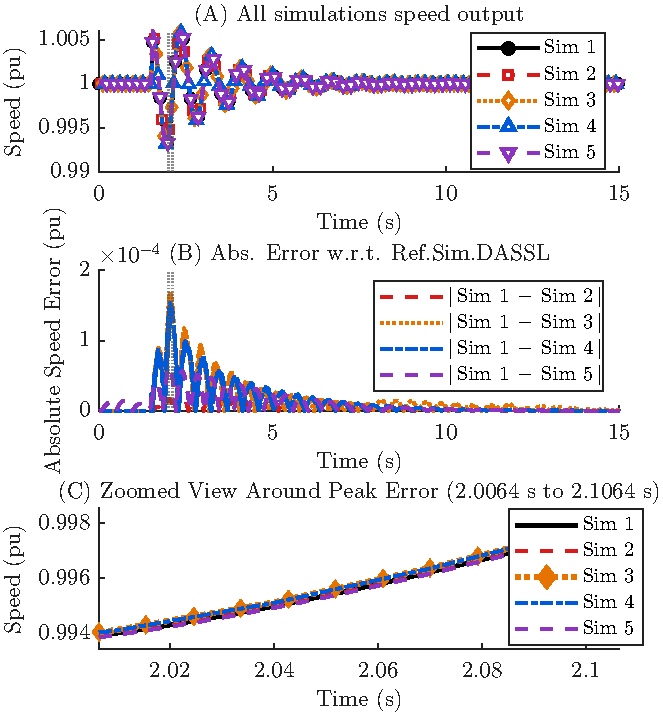
\includegraphics[width=0.95\columnwidth]{./figures/sec03_fig4_all_cases_vs_baseline.pdf}}
    \vspace{-2ex}
    \caption{MiL Simulations: (A) \texttt{w} for all simulations (see Figure \ref{fig:genunit}~(D)), (B) $\forall{i}\in\{2,3,4,5\}:\;\left|\right.$\texttt{Ref.Sim.DASSL}$\;-\;$Case$\;i\left.\right|$, (C) Zoomed view around peak error.}
    \label{fig:milsims}
    \vspace{-2ex}
\end{figure}

\begin{table}[t!]
    \centering
    \caption{Generator speed error relative to \texttt{Ref.Sim.DASSL}.}
    \vspace{-2ex}
    \label{tab:milstats}
    \small
\begin{tabular}{@{} c S[table-format=1.4e-1] S[table-format=1.4e-1] c @{}}
\toprule
Case & {max $|\epsilon|$ (pu)} & {RMS $\epsilon$ (pu)} & {$t_{\max}$ (s)} \\ \midrule
2    & 3.0160e-05            & 9.2302e-06            & 3.2156           \\
3    & 1.6949e-04            & 3.0662e-05            & 2.0564           \\
4    & 1.5353e-04            & 2.7456e-05            & 2.0564           \\
5    & 6.1989e-05            & 1.6466e-05            & 2.0310           \\ \bottomrule
\end{tabular}
    \vspace{-2ex}
\end{table}

The subsequent step to further refine the level of detail in our representation of the CHiL configuration is to generate eFMUs for \emph{both} the \controller{} \emph{and} the \plant{}, and then employ these in place of the \texttt{pss} and \texttt{G4CHIL} models as illustrated in Figures~\ref{fig:chilmodels}(C) and (D) to conduct SiL tests of the generated eFMI production code.

\section{Generation \& SiL testing of eFMUs}\label{sec:efmuGenAndSiL}

To generate eFMUs for the PSS and power system variants that have been designed and MiL-tested in Section \ref{sec:modeling-for-mil-testing}, Dymola offers the \texttt{DymolaEmbedded} library. It features a convenient user interface---graphical in the diagram and parameter editor views, yet also fully scriptable in \texttt{*.mos} files like any other Modelica library in Dymola---for configuring eFMU generation and conducting SiL tests of the resulting ISO/IEC 9899 (C11, C17, or C24 compliant) production code.

The production code of exported eFMUs leverages on the GALEC guarantees sketched in Section \ref{sec:efmi-standard}; in particular, Dymola's whole range of symbolic equation system optimizations are automatically conducted to find an algorithmic, inline-integrated eFMI GALEC solution for models subject to eFMU export.

\subsection{eFMU configurations}\label{sec:eFMU-configurations}

\begin{figure}[b!]
    \centerline{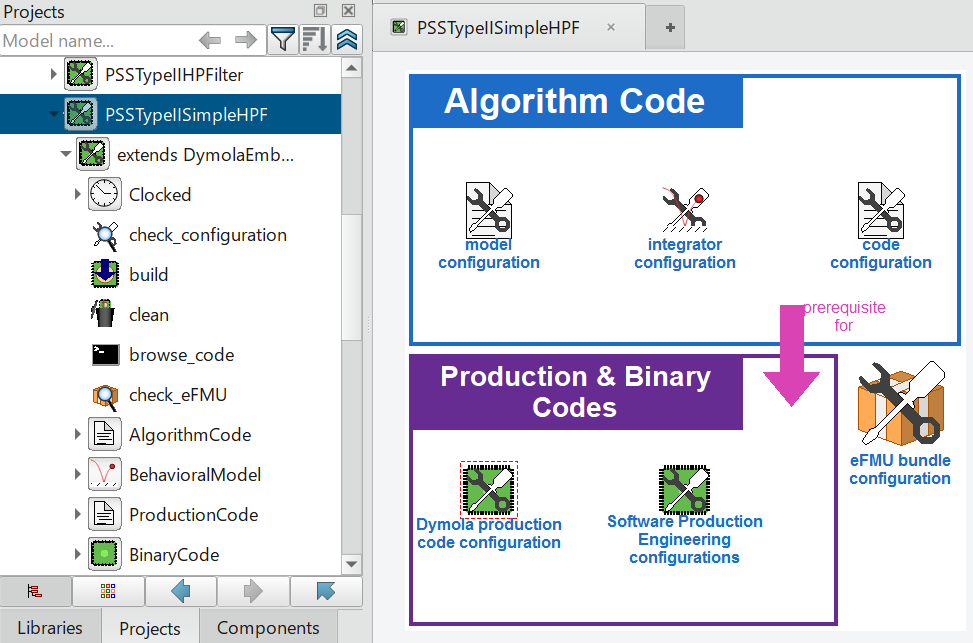
\includegraphics[width=0.99\columnwidth]{./figures/eFMU-configuration.png}}
    \vspace{-2ex}
    \caption{\texttt{DymolaEmbedded} eFMU configuration for the PSS \controller{} of Figure \ref{fig:pssvariants}~(D). Double-clicking on diagram-view components opens the respective configuration. Calling functions of the \textit{extends}-entry in the package browser executes the respective action, e.g., building GALEC or production code or analyzing code quality with clang-tidy or Cppcheck Premium.}
    \label{fig:eFMU-configuration}
    %\vspace{-4ex}
\end{figure}

To configure eFMU export for a Modelica model, a new package extending \texttt{DymolaEmbedded.EmbeddedConfiguration} has to be created. Each such extending-package represents an eFMU configuration and inherits configuration options and generative facilities as shown in Figure \ref{fig:eFMU-configuration}. The available configuration options are as follows:

\squishlist
    \item \textit{eFMU bundle configuration:} Optional name of the directory that shall contain the generated eFMU. If not explicitly set, the full qualified package name of the eFMU configuration is used.
    \item \textit{Model configuration:} Model subject to eFMU export (mandatory).
    \item \textit{Integrator configuration:} Fixed sampling period (mandatory) and optional solver method for inline-integration. The only mature solver currently supported is the explicit Euler method; implicit Euler and Rosenbrock methods~\cite{Olsson2017Rosenbrock} are still at the prototype stage for eFMU export.
    \item \textit{Code configuration:} Optional options to obfuscate generated GALEC code, constant-fold all parameters to reduce code size (parameters are hard-coded in the generated code rather than exposed through the GALEC block interface; dependent parameters are removed, preventing any later recalibration), and keep multi-dimensional entities intact rather than reducing them to scalars (e.g., used to preserve tensor-flows of embedded neural networks modeled using the \texttt{NeuralNetworks} package of the \texttt{eFMI} library, cf. \cite{Kamp2025}).
    \item \textit{Software Production Engineering configurations:} Preconfigured production code generator settings. Defines the floating-point precisions for which production codes shall be generated (by default for 32-bit and 64-bit)---these are the eFMU Production Code containers to generate. Also defines for which instruction set architectures (by default for x86, Microsoft\regtm{} Windows\regtm{} 32- and 64-bit) statically linked libraries shall be generated for each Production Code container---these are the eFMU Binary Code containers used for SiL simulation within Dymola (cf. Section \ref{sec:modelica-based-sil-tests}).
    \item \textit{Dymola production code configuration:} Deprecated embedded code export, predating Dymola's eFMI support.
\squishend

\noindent{}For the PSS and power system variants designed in Sections \ref{sec:pss-models} and \ref{sec:power-system-models}, an explicit Euler with a 0.2 ms sampling period is set as the integrator configuration. In addition, the \controller{} of Figure \ref{fig:pssvariants}~(D) and the \plant{} of Figure \ref{fig:g4chil} are chosen as model configurations, respectively. For both, code obfuscation is deactivated.

The generative facilities (i.e., inherited functions) provided by eFMU configurations are:

\squishlist
    \item \texttt{build()}: Generate eFMU with Algorithm, Production and Binary Code containers. Optionally also export SiL-stubs (cf. Section \ref{sec:modelica-based-sil-tests}) and source code FMUs for each generated Production Code container (cf. Section \ref{sec:production-code-export}). The root-level \texttt{build()} function exists for convenience; each eFMU container can be individually generated within the \texttt{build()} functions of the respective sub-packages (e.g., \texttt{ProductionCode.build()}).
    \item \texttt{browse\_code()}, \texttt{clean()}: Open the eFMU in the default file manager or shell (e.g., File Explorer and \texttt{cmd} in Microsoft Windows); delete all generated artifacts.
    \item \texttt{ProductionCode.check\_codes()}: Analyze Production Code containers with clang-tidy and Cppcheck Premium (cf. Section \ref{sec:production-code-quality-analyses}) for code quality and MISRA C:2023 compliance.
    \item \texttt{build\_FMUs()}, \texttt{build\_Simulink\_imports()}, and \texttt{build\_Arduino\_sketches()} of \texttt{ProductionCode}: Export Production Code containers as source code co-simulation FMUs, Simulink\regtm{} C Function blocks or Arduino\regtm{} sketches (cf. Section \ref{sec:production-code-export}), respectively.
    \item \texttt{BehavioralModel.build\_tests()}: Reuse existing Modelica experiments to derive SiL-tests for the production codes of the eFMU (cf. Section \ref{sec:modelica-based-sil-tests}).
\squishend

\noindent{}By default (i.e., if arguments are not interactively changed), the above generative eFMU facilities work with the options of their respective eFMU configuration (i.e., the \texttt{DymolaEmbedded.EmbeddedConfiguration} modifiers of their call context). Hence, it is not necessary to reconfigure eFMU export repeatedly when switching models or libraries; instead, configurations are stored together with their corresponding eFMU configuration package.

Note that being ordinary Modelica packages, eFMU configurations (their options and functions) can be scripted in Modelica \texttt{*.mos} scripts. This enables convenient configuration of variants and batch processing. Likewise, an \textit{eFMI}-button in Dymola's \textit{Tools}-ribbon (see Figure \ref{fig:eFMI-tools-ribbon-button}) enables the user to build all eFMUs of a whole package hierarchy, or load the SiL-stubs of existing eFMUs.

\begin{figure}[h!]%\centerline{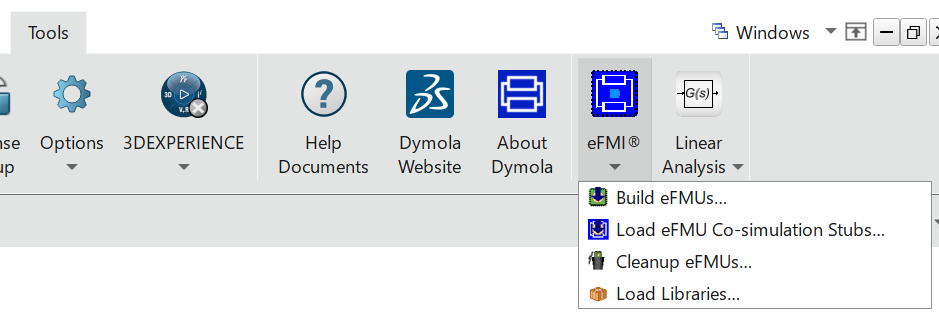
\includegraphics[width=0.95\columnwidth]{./figures/eFMI-tools-ribbon-button.png}}
\centerline{\includesvg[width=1.0\columnwidth]{./figures/eFMI-tools-ribbon-button.svg}}
    \vspace{-2ex}
    \caption{\textit{eFMI}-button in Dymola's \textit{Tools}-ribbon.}
    \label{fig:eFMI-tools-ribbon-button}
    \vspace{-2ex}
\end{figure}

\subsection{Modelica-based SiL tests}\label{sec:modelica-based-sil-tests}

\paragraph{SiL experiment packages:} To validate the functional correctness of the production codes generated for \controller{} and \plant{} models, we reused the MiL experiments of Section \ref{sec:mil-tests} as a basis to define respective SiL tests. To that end, Dymola's eFMI facilities support the generation of SiL experiment packages backed by an eFMI Behavioral Model container derived from an existing Modelica experiment; the \texttt{BehavioralModel.build\_tests()} function of an eFMU configuration (cf. Section \ref{sec:eFMU-configurations}) can be used to generate such SiL experiment packages. Given any Modelica experiment model, \texttt{build\_tests()} extracts---based on the \textit{model configuration} of the eFMU configuration in whose context it is executed---all instances of the model subject to eFMU code generation. Each instance defines a test scenario. 

\begin{figure}[t!]
    \centerline{\includesvg[width=1.0\columnwidth]{./figures/SiL-test-2.svg}}
    \vspace{-2ex}
    \caption{(A) SiL experiment package derived from the MiL experiment of Figure \ref{fig:refsim}, (B) SiL test model for the 32-bit floating-point precision production code generated for the PSS \controller{} of Figure \ref{fig:pssvariants}~(D).}
    \label{fig:SiL-test}
    \vspace{-2ex}
\end{figure}

Figure \ref{fig:SiL-test}~(A) shows the SiL experiment package (\texttt{SiLTest}) generated from the MiL experiment of Figure \ref{fig:refsim} for the \controller{} of Figure \ref{fig:pssvariants}~(D). The \texttt{Test\_ReferenceExperiment} model exploits the MiL experiment of Figure \ref{fig:refsim} to record reference trajectories. The \texttt{Test\_SiL\_} models are for testing the various production codes of the eFMU. The \texttt{build()} function simulates \texttt{Test\_ReferenceExperiment} and generates the Behavioral Model container backing the SiL experiment package, in particular its comma separated value (CSV) files with the reference trajectories and a manifest file with meta-information about the test scenarios, their in- and outputs, their respective units, etc. The \texttt{browse\_container()} function just opens the backing Behavioral Model container in the default file manager (e.g., File Explorer in Microsoft Windows).

\paragraph{SiL test models:} Figure \ref{fig:SiL-test}~(B) shows the SiL test model for the 32-bit floating-point precision production code for the \controller{} of Figure \ref{fig:pssvariants}~(D). The \texttt{eBlock} component is a SiL-stub generated for the production code. Such stubs are Modelica models with the same interface as the source model of an eFMU configuration, but their implementation is done by referencing the eFMU's production code by means of Modelica's external C code interface (the concept is similar to the Modelica stubs Dymola generates for imported FMUs). The \texttt{\textquotesingle{}vSI|table\textquotesingle{}} and \texttt{\textquotesingle{}vs|table\textquotesingle{}} components are input tables providing the reference trajectories for the PSS. The \texttt{\textquotesingle{}vs|match\textquotesingle{}} block simply compares the actual \texttt{vs} output of the production code (\texttt{eBlock.vs}) with the expected reference trajectory considering user-defined absolute and relative tolerances. The used tolerances can be defined for all scenarios, or specific ones, in the root diagram view of generated SiL experiment packages; they are the only additional user input required. Otherwise, the whole SiL experiment package can be generated from the MiL experiment of Figure \ref{fig:refsim}.

All components, except the \texttt{eBlock}, are from the \texttt{Testing}\footnote{\tiny{\url{https://www.youtube.com/watch?v=wnk5YbEgTjM}}} Modelica library, freely available with Dymola. \texttt{Testing} is a professional library to exploit Modelica experiments for testing purposes, automate regression tests (e.g., with Jenkins\footnote{\tiny{\url{https://www.jenkins.io/}}}), and provide convenient test results and plots. It is used for the continuous integration tests of the commercial Modelica library portfolio of Dassault Systèmes.

\paragraph{SiL test results:} The results of the SiL tests for our eFMUs are satisfactory. For the \controller{} of Figure \ref{fig:pssvariants}~(D), the \texttt{vs} output of the 32-bit floating-point precision production code has a maximum deviation of ${\approx}0.000365324$ for the test scenario of Figure \ref{fig:refsim} (note that the reference trajectories are recorded based on 64-bit floating-point precision simulations); the 64-bit production code has a maximum deviation of ${\approx}1.38778e-16$. The \texttt{w} output of the \plant{} of Figure \ref{fig:g4chil} has deviations as follows: ${\approx}0.000161166$ for 32-bit floating-point precision production code and ${\approx}-1.77636e-14$ for 64-bit.

Note that we will system integrate the 32-bit production codes in Section \ref{sec:STM32-integration-of-eFMUs} since the \controller{} STM32 board (NUCLEO-L476RG) supports hardware acceleration only for 32-bit floating-point precision and 64-bit floating-point precision production code for the \plant{} turned out to execute significantly slower on its STM32 board (NUCLEO-H723ZG) than the 32-bit floating-point precision code, leaving to little headroom with a very high risk of overruns in case of merely minor future model changes (cf. Section \ref{sec:results-and-analyses} for details).

\subsection{Production code quality analyses}\label{sec:production-code-quality-analyses}

To validate that eFMU production code generated by Dymola is of very high quality, Dymola provides preconfigured code quality checks with clang-tidy\footref{fnt:clang-tidy} and Cppcheck Premium\footref{fnt:cppcheck-premium}; the latter is particularly useful to validate MISRA C:2023 compliance. The preconfigurations are as verbose, complete and strict as possible.

\paragraph{Clang-tidy configuration:} For clang-tidy all checks are enabled except the following checks: (1) \textit{readability-identifier-length} (disabled because names of source Modelica models shall be reused, but in physics often very short variable names are used like \texttt{v} for voltage or \texttt{w} for rotational speed), (2) \textit{cppcoreguidelines-avoid-magic-numbers} and \textit{readability-magic-numbers} (physics equations can contain magic numbers), (3) \textit{altera-unroll-loops} and \textit{altera-id-dependent-backward-branch} (loop unrolling shall be done by the compiler, not the user; the implementation of multi-dimensional GALEC functions in generated production code is universal---their loops depend on the passed size arguments but these are literals at the call site, which is why we can assume compilers are capable of automatic optimization), and (4) \textit{altera-struct-pack-align} (code shall be portable and alignment automatically handled by the compiler).

\paragraph{Cppcheck Premium configuration:} For Cppcheck Premium the check-level is exhaustive, including style and information analyses; even inconclusive analyses are reported. Further MISRA C:2023 and SEI CERT C Coding Standard\footref{fnt:sei-cert-c} checks are enabled. For the implementation of GALEC built-in functions, a dedicated library configuration is provided to help Cppcheck identify built-in function API violations (e.g., if passed pointers to multidimensional variables must already be allocated and/or initialized).

\begin{figure*}[t]
    \centerline{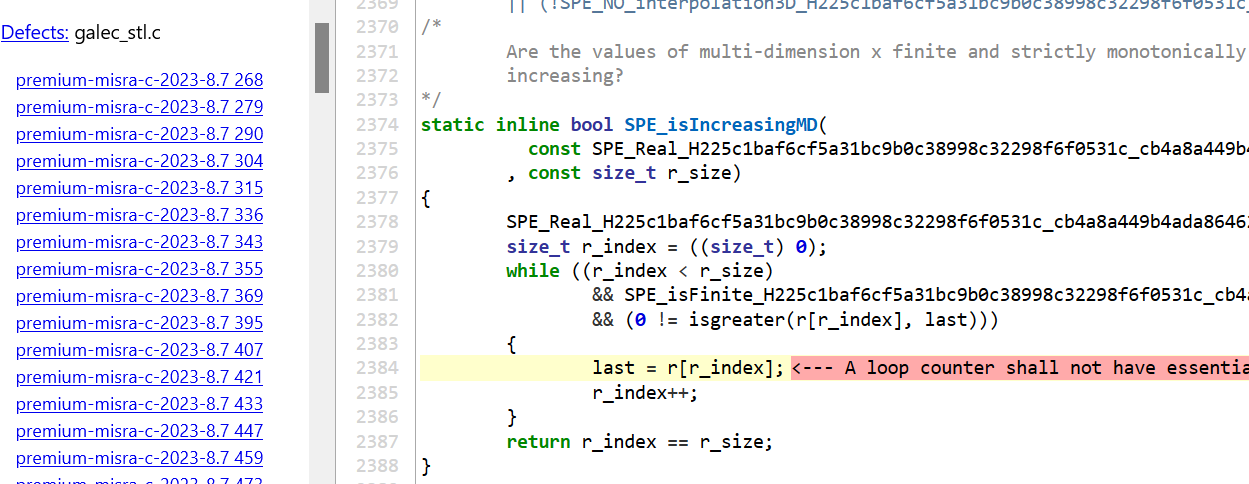
\includegraphics[width=1.5\columnwidth]{./figures/Cppcheck-report.png}}
    \vspace{-1ex}
    \caption{Excerpt of the Cppcheck Premium report for the 32-bit floating-point precision production code generated for the PSS \controller{} of Figure \ref{fig:pssvariants}~(D).}
    \label{fig:Cppcheck-report}
    \vspace{-2ex}
\end{figure*}

\paragraph{Code analyses results:} The results of the production code analyses for our examples can be found in the public repository\footref{fnt:pss-repository}; for each production code container in the \texttt{logs/check-code/clang-tidy} and \texttt{Cppcheck} subdirectories respectively. In the following discussion, we consider the 32-bit floating-point precision code for the \controller{} of Figure \ref{fig:pssvariants}~(D).

First of all, clang-tidy (Clang Tools 19.1.5) reports that 64-bit floating-point precision literals are assigned to 32-bit variables (\textit{bugprone-narrowing-conversions} and \textit{cppcoreguidelines-narrowing-conversions} violations); this is a shortcoming of Dymola's production code generator, which fails to add proper \texttt{F} suffixes, like in \texttt{1.0F / instance->wscale}. Note however, that the actual literals stem from the source model where they are in 64-bit precision. The narrowing when generating 32-bit floating-point precision production code is intended, but we fail to make it explicit to avoid  the reports. Further, clang-tidy reports that some local variables are not initialized (\textit{cppcoreguidelines-init-variables} violations), which, after manual inspection, are clearly false-positive reports. There are no further reports by clang-tidy.

The Cppcheck Premium 26.3.0 reports are much more interesting. They are syntax highlighted using Python Pygments\footnote{\tiny{\url{https://pygments.org/}}}, as shown in Figure \ref{fig:Cppcheck-report}. There are 204 reported issues, most are systematic false-positives considering our application. There are 159 violations of MISRA C:2023 Rule 8.7 (advisory), \textit{"Functions and objects should not be defined with external linkage if they are referenced in only one translation unit"}; all are about GALEC built-in functions, whose implementation is intended as shared library---hence, can be ignored. There are 23 violations of SEI CERT C DCL06-C, \textit{"Use meaningful symbolic constants to represent literal values"}; they stem from magic-numbers in physics equations---hence, can be ignored too. There are 3 violations of SEI CERT C INT30-C, \textit{"Ensure that unsigned integer operations do not wrap"}, which we know to be false-positives because the respective \texttt{index - 1} expressions can become at most 0 due to indexing starting at 1 in eFMI GALEC. All other reported issues fall into one of these categories, like a \texttt{typedef} or objects intended for library usage (MISRA C:2023 Rule 2.3 \& 8.9 (advisory) violations). The only interesting MISRA C:2023 violation reported is for Rule 14.1 (required), \textit{"A loop counter shall not have essentially floating type"}, which has been reported for a function deciding if an array only contains strictly increasing values (used to define an interpolation abscissa); this report is a false-positive the Cppcheck team meanwhile fixed in Cppcheck Premium 26.6.0 based on our findings.

\subsection{Production code export}\label{sec:production-code-export}

In general, Dymola-generated production code can be integrated into an embedded system with little effort, as will be illustrated for the STM32 ecosystem in Section~\ref{sec:stm32-system-integration-main-loop}. Nevertheless, Dymola supports dedicated production code export for popular embedded ecosystems. Export/import thereby means to use the C code of an eFMU Production Code container as is, add any required wrapper code and meta-information to satisfy target ecosystem API requirements, and import the code such that the further (in particular compilation) infrastructure of the target ecosystem can be used for system integration on actual hardware. Dymola supports export of production code for (the respective eFMU configuration facilities are listed in Section~\ref{sec:eFMU-configurations}):

\squishlist
    \item \textit{FMI\regtm{}:} Export as FMI\footref{fnt:fmi} 3.0 source code co-simulation FMU with \texttt{fixedInternalStepSize}. The only code added to exported production code, besides the mandatory \texttt{modelDescription.xml}, is the required implementation of \texttt{fmi3Functions.h}, which is lean, avoiding as much overhead of the generic FMI interface as possible while at the same time introducing sanity checks to ensure the FMU is used as intended (in particular called with its fixed sampling period or a proper multiple thereof). eFMU production code exported as source code FMU enables the use of eFMI on many dedicated real-time platforms with source code FMU import; the tooling of such platforms will take care of compiling and deploying the production code. Examples are ConfigurationDesk\regtm{} (dSPACE), TwinCAT\regtm{} (Beckhoff\regtm{}), or Silver\regtm{} (Synopsys\regtm{}).
    
    It is noteworthy that the eFMU production code based FMUs exported by Dymola are significantly smaller than FMUs exported with its normal source and binary code co-simulation FMU export. For the \controller{} of Figure \ref{fig:pssvariants}~(D) the eFMU production code backed source code FMU is ${\approx}31$ kB, its compiled binary code version for Microsoft Windows 11 64-bit on Intel\regtm{} x86-64 is ${\approx}176$ kB, whereas the model directly exported as source code FMU is ${\approx}5.41$ MB and binary code FMU is ${\approx}2.84$ MB (in both cases exported with protected variables excluded, only black box, FMI 3.0 co-simulation, and inline integration method explicit Euler). Likewise for the \plant{} of Figure \ref{fig:g4chil}: ${\approx}38$ kB for the eFMU backed source code FMU, ${\approx}220$ kB for the eFMU backed binary code FMU, ${\approx}5.49$ MB for the normal source code FMU, and ${\approx}2.93$ MB for the normal binary FMU.
    \item \textit{Simulink:} Generate a MATLAB\regtm{} script, that when executed on a Simulink C Function block instantiates it to execute the respective production code. The GALEC block-interface (and therefore in-, outputs and parameters of the production code) are properly typed with native Simulink embedded real-time target (ERT) types such that unnecessary type conversions can be avoided; as is any copying of multidimensions. The resulting block can be used, and combined in Simulink like any other block. ERT code generators will take care of proper system integration of the C Function block, but otherwise use its backing eFMU production code as is (i.e., skip code generation for it).
    \item \textit{Arduino:} Exports production code as Arduino sketch, adding the required \texttt{*.ino} file with initialization and main loop as well as commented code where to access inputs, outputs, and parameters. Exported sketches are ready for further development and deployment via the Arduino IDE, or any other Arduino compatible tooling.
\squishend

\noindent{}For all export/import options the high-quality standards of eFMU production code as generated by Dymola are preserved, including being free of additional library dependencies besides common C Standard Library routines (mostly \texttt{math.h}).

\section{STM32 integration of eFMUs}\label{sec:STM32-integration-of-eFMUs}

The \controller{} and \plant{} eFMUs generated in Section \ref{sec:efmuGenAndSiL} still need to be system integrated on physical microcontrollers. The STM32 (STMicroelectronics\regtm{}) ecosystem has been used as the target here since it is widely-used, low-priced, and well-documented with good development and software support. Being mainly a hardware manufacturer---and as often the case in the embedded domain---STMicroelectronics' viewpoint starts from the hardware and not the model. System integration starts with the selection of one of the target microcontrollers in STM32CubeMX, where peripherals like GPIO pins, DACs, and timers are configured, with template code ultimately being generated, initializing and provisioning all configured peripherals based on the hardware abstraction layer (HAL), lower-layer (LL) drivers, and Arm\regtm{} Cortex\regtm{}-M CMSIS provided by the used STM32CubeH7 software package managed\footnote{STM32CubeMX proposes a catalog of locally installed and online available STM32CubeH7 versions suited for the target microcontroller.} in STM32CubeMX. The result of STM32CubeMX template generation is a C development project for STM32CubeIDE, whose \texttt{main()} execution routine (\texttt{int main(void)} function in \texttt{main.c}) is ready for adding the actual user-code interacting with the configured peripherals. In our case, eFMI system integration therefore means to integrate the 32-bit floating-point precision production codes of the \controller{} and \plant{} eFMUs into the \texttt{main()} execution routines of their respective template codes generated by STM32CubeMX. Note the plural; \controller{} and \plant{} have their individual STM32CubeIDE projects.

A direct STM32 system integration not using tooling like STM32CubeMX and STM32CubeIDE would be possible too, but that requires professional knowledge we consider rare in our development process, which is driven by the modeling community; it also would be a laborious task not paying off for sporadic use-cases.

\subsection{Board configuration with STM32CubeMX}\label{sec:STM32CubeMX}

\paragraph{Hardware configuration:} Two STM32 Nucleo-64/144 boards were chosen for deploying the eFMU production codes developed in Section \ref{sec:efmuGenAndSiL}. A NUCLEO-L476RG was used to deploy the \controller{}, where the system clock of 80 MHz was sufficient to support real-time evaluation of the model. A NUCLEO-H723ZG was selected to run the \plant{}. The much higher 550 MHz system clock is preferable for performing the fast matrix algebra required by the corresponding production code. Both the NUCLEO-L476RG and the NUCLEO-H723ZG have (at least) one analog input (ADC) and one analog output (DAC) for mapping the input and output signals.

\paragraph{Pin configurations:} The analog and digital I/O must be mapped to prevent peripheral collisions and minimize latency during the 5 kHz execution loop (i.e., 0.2 ms sampling period). Digital LEDs are employed to signal real-time violation and production code errors, whereas digital output pins are enabled to examine execution times through an oscilloscope by means of low/high voltage toggling at each sampling point and a separate high-voltage signal whenever eFMU production code is in execution. Digital inputs, such as the onboard push-button for the manually controlled \plant{} fault condition trigger, were also mapped in the STM32CubeMX configuration. For example, for the NUCLEO-H723ZG used for the \plant{}, the primary analog input (the voltage output of the PSS \controller{} board) was assigned to GPIO pin \texttt{PA3}, corresponding to ADC1 channel 15; and the calculated speed output ($\omega$) was assigned to GPIO pin \texttt{PA5}, which connects directly to the DAC1 output channel. A similar approach was taken for the \controller{} I/O configuration, whose NUCLEO-L476RG pin configuration is shown in Figure \ref{fig:cubemx-pin-config}.

\begin{figure}[t!]
    \vspace{-4ex}
    \centerline{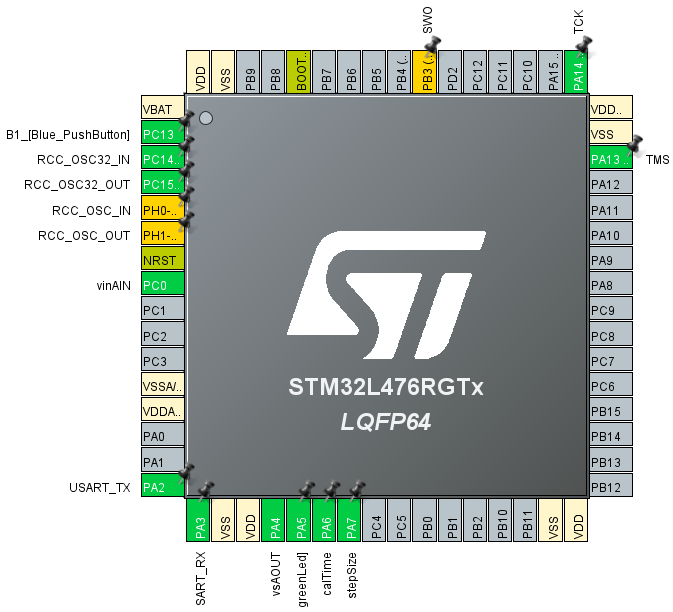
\includegraphics[width=0.9\columnwidth]{./figures/CubeMX_Pins.png}}
    \vspace{-2ex}
    \caption{STM32CubeMX pin configuration for the NUCLEO-L476RG used as the \controller{}.}
    \label{fig:cubemx-pin-config}
    \vspace{-2ex}
\end{figure}

We also prototyped more advanced plant models supporting variable loads via an additional input that can be interactively changed with a potentiometer\footnote{Although not further discussed for space considerations, the variable-load variant has been successfully deployed and tested.}. In that case, the additional analog input has been deliberately mapped to GPIO pin \texttt{PC0} because it can physically route to an entirely independent analog-to-digital converter, ADC2 (specifically \texttt{ADC123\_INP10}). Distributing the analog input signals across separate, dedicated ADCs avoids the need for complex ``Scan Mode'' channel switching or Direct Memory Access (DMA) pipelines. This hardware-level isolation ensures deterministic, low-latency sampling within the tight 0.2 ms timer interrupt.

\paragraph{Clock configurations:} In Dymola, the sampling period of eFMU configurations is explicitly set (see Section \ref{sec:eFMU-configurations}). For the STM32CubeMX configurations, the clock dividers and pre-dividers must be calculated to match the exact sampling period set in the eFMU. The timer's clock rate (its frequency) is determined by the following equation:

\begin{equation*}
    \text{frequency} = \frac{\text{APB Clock}}{(\text{ARR}+1)(\text{PSC}+1)}
\end{equation*}

\noindent{}where ARR stands for Auto-Reload Register and PSC stands for the timer's prescaler. The APB Clock is the system clock that has been pre-divided for the peripherals (such as timers). The limitations of the ARR and prescaler will be displayed in the STM32CubeMX GUI. 

For example, the embedded board that is used as the \plant{} is required to sample every 0.2 ms (i.e., at 5 kHz frequency). To this end, the NUCLEO-H723ZG, which has a 550 MHz system clock, is configured to have an APB pre-divider of 2, an ARR of 199, and a PSC of 274. That results in the desired frequency:

\begin{equation*}
    \text{frequency} = \frac{550/2 \text{ MHz}}{(199+1)(274+1)} = 5 \text{ kHz}
\end{equation*}

\noindent{}These clock configuration parameters are set in the timer peripheral menu of STM32CubeMX. For the \plant{} board, TIM2 was used with the parameters found above, as shown in Figure \ref{fig:cubemx-timer-config}.

The timer configuration for the \controller{} is likewise, except that TIM1 is used instead of TIM2 and that its APB Clock, ARR, and PSC values are different to achieve a 0.2 ms sampling period because the NUCLEO-L476RG has a 80 instead of a 550 MHz Arm Cortex-M processor.

\begin{figure}[t!]
    \centerline{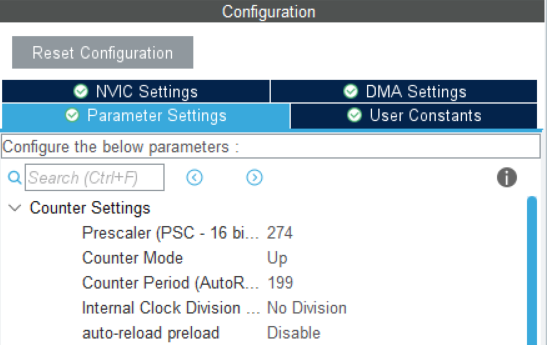
\includegraphics[width=0.9\columnwidth]{./figures/CubeMX_TIM2Config_H723.png}}
    \caption{SMT32CubeMX timer configuration for the NUCLEO-H723ZG used as the \plant{}.}
    \label{fig:cubemx-timer-config}
    \vspace{-2ex}
\end{figure}

\paragraph{Code generation configurations:} To maintain a clean file structure---in particular for the generated \texttt{main()} execution routine in \texttt{main.c}---the code generator of STM32CubeMX was set to generate peripheral initialization as a pair of \texttt{.c/.h} files per peripheral. The respective setting is in Project Manager $\rightarrow$ Code Generator $\rightarrow$ ``Generate peripheral initialization as a pair of \texttt{.c/.h} files per peripheral''. Additionally, the target IDE was set to STM32CubeIDE under Project Manager $\rightarrow$ Project $\rightarrow$ Toolchain/IDE.

\paragraph{Generated template code overview:} The template code generated by STM32CubeMX serves as the foundational bare-metal layer for the microcontrollers. Upon boot, the code initializes the ARM Cortex-M processor and configures the system clock tree to drive the NUCLEO-H723ZG at 550 MHz and the NUCLEO-L476RG at 80 MHz. The GUI shows which specific GPIO pins can be mapped to ADC and DAC channels, and initializes the hardware timers using the ARR and PSC values calculated to ensure that the timer interrupts fire at the exact 5 kHz rate required by each of the sampling periods configured in Section \ref{sec:eFMU-configurations}. In addition, initialization code for the HAL is generated. Because the eFMU's production code is system integrated into the generated template code, it is critical that all custom logic, like eFMU function calls, is placed strictly within the designated \texttt{/* USER CODE BEGIN /} and \texttt{/ USER CODE END */} tags; otherwise, code regeneration during subsequent hardware reconfigurations would overwrite the manually added production code integration.

\subsection{Programming, compilation, and deployment with STM32CubeIDE}\label{sec:STM32CubeIDE}

\paragraph{eFMU production code inclusion:} Rather than manually copying the production codes generated for the \controller{} and \plant{} into their respective STM32CubeIDE projects, the Production Code containers of the respective eFMUs were symbolically linked using relative paths based on project environment variables provided by STM32CubeIDE (e.g., \texttt{PARENT-3-PROJECT\_LOC} for the level-3 parent directory of the project root directory). This allows the \controller{} and \plant{} Modelica source models to be iteratively tweaked and re-exported from Dymola as eFMUs without requiring manual production code re-import in their respective STM32CubeIDE projects (just refreshing the projects is sufficient)---an important feature for iterative, rapid prototyping cycles from a Modelica model to deployable embedded code. Besides symbolic linking, the eFMU production codes also have to be added to the list of include and source file directories such that STM32CubeIDE takes care of their compilation and binary code generation.

\paragraph{Manual system integration in \texttt{main.c}:}\label{sec:stm32-system-integration-main-loop}

Manual coding to system integrate the eFMU production codes is only required in the \texttt{main.c} files generated by STM32CubeMX. The required steps are very similar for the \controller{} and \plant{} and are explained in the following by the example of the \controller{}.

First, the eFMU production code must be included via \texttt{\#include "block.h"} to enable \controller{} initialization, recalibration, and sampling via the eFMI GALEC block-interface routines \texttt{Startup()}, \texttt{Recalibrate()}, and \texttt{DoStep()}. Note that the implementation generated by Dymola uses hashed names, such that name clashes when several eFMUs are compiled and linked together are avoided. This is not required in our example---after all \controller{} and \plant{} are individual STM32CubeIDE projects deployed on individual boards---for which reason we can introduce simplified names via \texttt{\#define} preprocessor macros that ease the readability of subsequent system integration code:

\begin{lstlisting}[
    language = c,
    caption={},
    label={lst:main-1}]
/* USER CODE BEGIN Includes */
#include "block.h"
/* USER CODE END Includes */

/* USER CODE BEGIN PTD */
#define CONCAT_INNER(a, b) a##b
#define CONCAT(a, b) CONCAT_INNER(a, b)

/* Shortcut names for hash-based eFMU API: */
#define MODEL_HASH \
  H225c1baf6cf5a31bc9b0c38998c...

typedef CONCAT(BlockState_, MODEL_HASH) \
  ModelPSS;
typedef CONCAT(SPE_Real_, MODEL_HASH) \
  PSS_Real;
typedef CONCAT(SPE_ErrorSignal_, MODEL_HASH) \
  PSS_ErrorSignal;

#define PSS_NONE_ERRORSIGNAL \
  CONCAT(SPE_ERRORSIGNAL_NONE_, MODEL_HASH)
#define PSS_UNSPECIFIED_ERRORSIGNAL \
  CONCAT(SPE_ERRORSIGNAL_UNSPECIFIED_ERROR_, MODEL_HASH)

#define PSS_Startup \
  CONCAT(Startup_, MODEL_HASH)
#define PSS_DoStep \
  CONCAT(DoStep_, MODEL_HASH)
#define PSS_Recalibrate \
  CONCAT(Recalibrate_, MODEL_HASH)
#define PSS_Reinitialize \
  CONCAT(Reinitialize_, MODEL_HASH)
/* USER CODE END PTD */
\end{lstlisting}

\noindent{}Next, two global variables are introduced to capture sampling requests of the timer interrupt (\texttt{pending\_samplings}) and to engage or disengage the \controller{} interactively (\texttt{use\_pss}); the latter will be used in Section \ref{sec:results-and-analyses} to validate the stabilizing effects of the \controller{}:

\begin{lstlisting}[
    language = c,
    caption={},
    label={lst:main-2}]
/* USER CODE BEGIN PV */
/* Sampling request counter & PSS on/off button: */
static volatile uint8_t pending_samplings;
static volatile bool use_pss;
/* USER CODE END PV */
\end{lstlisting}

\noindent{}Note that both variables are \texttt{volatile} since they shall be changed by interrupt routines\footnote{There is no need for semaphores because the single core ARM Cortex-M processor guarantees atomic access for \texttt{uint8\_t} and \texttt{bool}.}; the \texttt{pending\_samplings} variable is changed whenever the timer interrupt triggers and \texttt{use\_pss} whenever the \texttt{B1} onboard button shown in Figure \ref{fig:wiring-diagram} is pressed. The interrupt routines we need to adapt are predefined by the STM32 HAL; \texttt{HAL\_TIM\_PeriodElapsedCallback} for the timer and \texttt{HAL\_GPIO\_EXTI\_Callback} for the onboard button:

\begin{lstlisting}[
    language = c,
    caption={},
    label={lst:main-3}]
/* USER CODE BEGIN 4 */
void HAL_TIM_PeriodElapsedCallback(
  TIM_HandleTypeDef *htim)
{
  /* Check for sampling timer interrupt: */
  if (TIM1 == htim->Instance)
  {
    if (((uint8_t) 255) > pending_samplings)
    {
      ++pending_samplings;
    }
    HAL_GPIO_TogglePin(
      stepSize_GPIO_Port,
      stepSize_Pin);
  }
}

void HAL_GPIO_EXTI_Callback(uint16_t GPIO_Pin)
{
  static uint32_t last_override = ((uint32_t) 0);

  /* Check for blue button (PC13) interrupt: */
  if (B1__Pin == GPIO_Pin)
  {
    const uint32_t current_time = HAL_GetTick();
    /*
      Debounce; only accept press if 250 ms
      passed since last:
    */
    if (((uint32_t) 250)
      < (current_time - last_override))
    {
      use_pss = !use_pss;
      last_override = current_time;
    }
  }
}
/* USER CODE END 4 */
\end{lstlisting}

\noindent{}The checks on Lines~6 and 23 are based on our STM32CubeMX \controller{} configuration for the timer (\texttt{TIM1}) and onboard button (\texttt{B1\_\_Pin}) peripherals, and ensure the action is only taken if the respective peripheral caused the interrupt. In case of the timer, we simply increase the \texttt{pending\_samplings} on Line~10 (ensuring it saturates instead of overflowing); in case of interactive \controller{} toggling we just invert \texttt{use\_pss} on Line~33 (incorporating a debounce time to avoid toggle-cascading).

We also flip a digital output on Lines~12-14 whenever the timer ticks. The resulting \texttt{stepSize} pulse signal---whose fixed-length is the sampling period---is useful for the computation time analyses of Section \ref{sec:results-and-analyses} since it provides a reference-grid for oscilloscope-based plots of the time required by the eFMU production code for computing individual samplings (cf. \texttt{calTime} of the control-loop listing below).

ARM Cortex-M interrupt routines have defined priority levels. Only routines of higher priority can interrupt others; pending interrupts of lower or equal priority are delayed until higher priority interrupts are complete. The logic of interrupt routines therefore should be concise to avoid interrupt overruns. For that reason, our timer interrupt only registers another sampling request in \texttt{HAL\_TIM\_PeriodElapsedCallback} instead of conducting the actual sampling (which would, in case of an overrun, silently block a following timer tick). The sampling code itself is within the control-loop of the interruptible \texttt{main()} execution routine:

\begin{lstlisting}[
    language = c,
    caption={},
    label={lst:main-4}]
/* USER CODE BEGIN WHILE */
while (true)
{
  /* USER CODE END WHILE */

  /* USER CODE BEGIN 3 */
  /* Conduct sampling if sampling timer ticked: */
  if (((uint8_t) 0) < pending_samplings)
  {
    /* Always reset the error signals: */
    error_signals = PSS_NONE_ERRORSIGNAL;

    /* Computation time for external profiling: */
    HAL_GPIO_WritePin(
      calTime_GPIO_Port,
      calTime_Pin,
      GPIO_PIN_SET);

    /* Input processing (convert AC to volt): */
    HAL_ADC_Start(&hadc1);
    if (HAL_OK == HAL_ADC_PollForConversion(
      &hadc1,
      POLL_TIMEOUT))
    {
      const uint32_t adc_raw =
        HAL_ADC_GetValue(&hadc1);
      pss.vSI =
        ((PSS_Real) adc_raw) * ADC_TO_VOLTS;
    }
    else
    {
      error_signals |= PSS_UNSPECIFIED_ERRORSIGNAL;
    }
    HAL_ADC_Stop(&hadc1);

    /* Compute sampling step: */
    PSS_DoStep(&pss);
    error_signals |= pss.ErrorSignals;

    /* Check if switch is pulling to GND: */
    const PSS_Real target_pu = use_pss
      ? pss.vs
      : CONSTANT_PU;

    /*
      Output processing (scaling, clamping,
      converting volt to AC):
    */
    PSS_Real dac_val =
      (target_pu + OFFSET) * VOLTS_TO_DAC;
    if (DAC_MIN > dac_val)
    {
      dac_val = DAC_MIN;
    }
    else if (DAC_MAX < dac_val)
    {
      dac_val = DAC_MAX;
    }
    HAL_DAC_SetValue(
      &hdac1,
      DAC_CHANNEL_1,
      DAC_ALIGN_12B_R,
      ((uint32_t) dac_val));

    /* Computation time for external profiling: */
    HAL_GPIO_WritePin(
      calTime_GPIO_Port,
      calTime_Pin,
      GPIO_PIN_RESET);

    --pending_samplings;
  }

  /* Set LED 2 for sampling errors or overruns: */
  if ((PSS_NONE_ERRORSIGNAL != error_signals)
    || (((uint8_t) 1) < pending_samplings))
  {
    error_timestamp = HAL_GetTick();
    HAL_GPIO_WritePin(
      LD2__GPIO_Port,
      LD2__Pin,
      GPIO_PIN_SET);
  }

  /*
    Unset LED 2 if on due to past errors
    (but always hold for at least 30000 ms):
  */
  if ((((uint32_t) 0) != error_timestamp)
    && (((uint32_t) 30000)
      < (HAL_GetTick() - error_timestamp)))
  {
    HAL_GPIO_WritePin(
      LD2__GPIO_Port,
      LD2__Pin,
      GPIO_PIN_RESET);
    error_timestamp = ((uint32_t) 0);
  }
}
/* USER CODE END 3 */
\end{lstlisting}

\noindent{}Note that the control-loop is greedy (\texttt{while (true)} on Line~2) instead of going to sleep until events happen; such ``busy waiting'' is typical for hard real-time code. It consists of three main parts: (1) On Lines~8-72, actual sampling---i.e., the use of eFMU production code to compute new outputs and internal control states for the given inputs and parameters---is conducted whenever the timer interrupt indicated a sampling point (\texttt{pending\_samplings} $\geq$ 1). (2) On Lines~75-83 errors---either (a) signaled by the block-interface functions of the eFMU production code (\texttt{error\_signals} variable set on Lines~37-38) or due to real-time violations, because of (b) non-timely input provision (timeout of \texttt{HAL\_ADC\_PollForConversion} on Lines~21-23) or (c) sampling computation overruns when the timer ticks again while a previous sampling still is processed (\texttt{pending\_samplings} $>$ 1 check on Line~76)---are detected and indicated by the onboard LED 2. (3) On Lines~89-98, LED 2 is reset if there have been no errors within the last 30 s.

Note that sampling on Lines~8-72 is mostly about input and output provisioning with respective timeout detection and AC/voltage conversions with scaling and clamping according to voltage ranges. The actual sampling logic is completely encapsulated in the eFMI \texttt{DoStep()} implementation of the eFMU production code (called on Line~37), which takes as argument a struct holding the current \controller{} state (\texttt{pss} holding the values of tunable and dependent parameters, in- and outputs, and states). The struct type is provided by the eFMU production code as is a respective eFMI \texttt{Startup()} implementation for its initialization. The only other noteworthy sampling actions are (1) to indicate the actual computation time with the \texttt{calTime} pulse signal (set to high-voltage when sampling starts on Lines~14-17 and reset on Lines~66-69 when it ends), (2) engage or disengage---not disable; just whether its output shall be used---the \controller{} on user request on Lines~41-43, and, of course, (3) reduce the sampling request counter on Line~71 when finished.

\paragraph{Compiler and linker settings:}

STM32CubeIDE provides various options for compilation and binary code generation. Our \controller{} and \plant{} projects each provide two predefined build configurations: A \textit{Debug} and a \textit{Release} build. Both share the following common settings (unmentioned options are left default):

\squishlist
    \item \textbf{MCU/MPU Toolchain:} The GNU Tools for STM32 (14.3.rel1) are used for compilation and binary code generation.
    \item \textbf{MCU/MPU Settings:} Use of the reduced C runtime library (\texttt{--specs=nano.specs}) and hardware-implemented floating-point ABI (\texttt{-mfloat-abi=hard}). For the NUCLEO-L476RG, where the \controller{} is deployed, its FPv4-SP-D16 floating-point unit is used; for the NUCLEO-H723ZG, its FPv5-D16 floating-point unit is used.
    \item \textbf{MCU/MPU GCC Assembler:} The preprocessor does not search system directories (\texttt{-nostdinc}) to avoid inclusion or configuration by external---third party set---macros.
    \item \textbf{MCU/MPU GCC Compiler:} Reports are verbose (\texttt{-v}). ISO C18 (\texttt{-std=c18}) is used as language standard to verify portability and compliance of the eFMU production code generated by Dymola. All warnings are enabled (\texttt{-Wall}, \texttt{-Wextra}, \texttt{-pedantic}, \texttt{-Wmissing-include-dirs}, \texttt{-Wswitch-default}, \texttt{-Wswitch-enum}, and \texttt{-Wconversion}). As expected from the production code analyses of Section \ref{sec:production-code-quality-analyses}, the eFMU production codes are free of any warnings except the 32-bit floating-point narrowing conversions already explained; interestingly, the driver/standard library implementation of STM32 has many warnings.
    \item \textbf{MCU/MPU GCC Linker:} Reports are verbose (\texttt{-v}). Standard libraries are not default included (\texttt{-nodefaultlibs}) and a minimal implementation for system calls is used (\texttt{--specs=nosys.specs}) to verify that the eFMI production code generated by Dymola is self-contained and without external library dependencies besides basic C Standard Library dependencies.
\squishend

\noindent{}The \textit{Debug} and \textit{Release} builds only differ in applied optimizations and available debug support:

\squishlist
    \item \textbf{MCU/MPU GCC Assembler:} The debug level is maximum (\texttt{-g3}) for the \textit{Debug} build and none for the \textit{Release} build; likewise for the MCU/MPU GCC Compiler settings, where additionally the \texttt{-DDEBUG} preprocessor directive is defined for the \textit{Debug} build but not for the \textit{Release} build.
    \item \textbf{MCU/MPU GCC Compiler:} The optimizations are none (\texttt{-O0}) for the \textit{Debug} build and most (\texttt{-O3}) for the \textit{Release} build. Stack usage analysis (\texttt{-fstack-usage}) and cyclomatic complexity (\texttt{-fcyclomatic-complexity}) are enabled for the \textit{Debug} build but not for the \textit{Release} build.
\squishend

\section{RT simulation and CHiL testing}\label{sec:rtchil}

All analyses in this section have been conducted with \textit{Release} builds if not mentioned otherwise explicitly (cf. Section \ref{sec:STM32CubeIDE}).

\subsection{CHiL experimental setup}

\paragraph{Schematics and wiring:} To perform CHiL tests, Figure \ref{fig:wiring-diagram} shows how the microcontrollers have been wired together along with an Analog Discovery 3\footnote{\tiny{\url{https://digilent.com/shop/analog-discovery-3/}}}, a multi-functional test and measurement device (labeled (M)). On the left hand side, the NUCLEO-L476RG, labeled (C), serves as the \controller{} running the PSS eFMU (from the model in Figure \ref{fig:pssvariants}~(D)), while on the right hand side the NUCLEO-H723ZG, labeled (P), acts as the \plant{} running the other eFMU (from the model in Figure \ref{fig:g4chil}).

\begin{figure}[h]
    \centerline{\includesvg[width=0.975\columnwidth]{./figures/setup-path.svg}}
    \vspace{-2ex}
    \caption{CHiL experimental setup wired to record measurement data from experiments using the Analog Discovery 3.}
    \label{fig:wiring-diagram}
    \vspace{-1ex}
\end{figure}

The speed output signal \texttt{w} of the \plant{}, in Figure \ref{fig:g4chil}, is now physically obtained from Figure \ref{fig:wiring-diagram}(P) (the NUCLEO-H723ZG) on pin \texttt{D13}. It is connected with a yellow wire to both the measurement channel \texttt{C1} of the Analog Discovery Board 3 (M) and to pin \texttt{A5} of the \controller{}, the NUCLEO-L476RG, labeled (C) in Figure \ref{fig:wiring-diagram}. Similarly, the output signal \texttt{vf} of the \controller{} in Figure \ref{fig:pssvariants}~(D)) is obtained from the NUCLEO-L476RG in Figure \ref{fig:wiring-diagram}(C) from pin \texttt{A2}. It is then connected with green wires to both the measurement channel \texttt{C2} of the Analog Discovery Board 3 and to pin \texttt{A0} of the \plant{}, the NUCLEO-H723ZG.

\paragraph{Interactive fault injection, stabilizer toggling, and resetting:} In traditional offline Modelica simulations, events like faults, reinitialization, or enabling or disabling a controller are typically triggered by absolute time components (e.g., the \texttt{faultTimer} in our offline simulation models of the CHiL setup, shown in Figure \ref{fig:chilmodels}). In a continuous HiL environment, absolute time based events are problematic however; there might be no well-defined, synchronized global clock for all devices, multiple consecutive test runs require synchronous resetting of all boards, and interactive testing is hampered. For these reasons, we decided for interactive, onboard button based, event triggering.

Manual \plant{} faults can be triggered by pushing the blue ``User Button'' on the NUCLEO-H723ZG, which is labeled \texttt{B1} on the bottom right of Figure \ref{fig:wiring-diagram}. Pressing the button pulls the GPIO pin high, instantly activating the fault dynamics of the \plant{} eFMU, while releasing it clears the fault, allowing for interactive, repeatable time-domain testing.

In case of the \controller{}, the corresponding ``User Button'' is configured to engage or disengage the eFMU itself. When the \controller{} button \texttt{B1}, on the left of Figure \ref{fig:wiring-diagram}, is pressed, it will ``turn-on'' the PSS, giving an output driven by the eFMU, and pressing it again will ``turn-off'' the PSS, giving a constant output.

Both boards, the L476RG and the H723ZG, can be individually reset using the buttons labeled \texttt{B2}, on the left hand side for the \controller{} and on the bottom right hand side for the \plant{}.

\paragraph{Analog Discovery 3 oscilloscope and network analysis:} The Analog Discovery 3 interfaces with Digilent's WaveForms\footref{fnt:waveforms} software package. This software is capable of acquiring oscilloscope measurements through two analog channels (see \texttt{C1} and \texttt{C2} in Figure \ref{fig:wiring-diagram}), allowing real-time analysis of the analog signals used by microcontrollers during experiments. Additionally, the Analog Discovery 3 includes a waveform generator, allowing for test signal injection into the Nucleo-64/144 boards so that their functionality could be tested independently. The WaveForms software also includes a network analysis tool, employing both the oscilloscope and waveform generator hardware features. This tool allows for the frequency dependent amplitude and phase responses of the circuit under test to be captured easily. This is achieved by connecting the waveform generator, \texttt{W1} in Figure \ref{fig:wiring-diagram}, and one analog probe, \texttt{C1}, to the input of the system, with the second analog probe, \texttt{C2} connected to the output of the system. Through this network analysis function, frequency response plots were generated and compared with the Bode plots generated by linearizing the Modelica models.

\paragraph{Full closed-loop network analysis setup:} Because the experimental CHiL setup includes two embedded boards in closed-loop, it is desirable to verify the frequency response characteristics of this closed-loop system as well. Figure \ref{fig:closed-loop-simulation} shows the Dymola model that was used to compare with the hardware-based closed-loop test.

\begin{figure}[t!]
    \centerline{\includesvg[width=0.95\columnwidth]{./figures/IOCL.svg}}
    \caption{Closed-loop model with input and output interfaces to compare with frequency response tests.}
    \label{fig:closed-loop-simulation}
    \vspace{-1ex}
\end{figure}

\begin{figure*}[t!]
    \centerline{\includesvg[width=1.5\columnwidth]{./figures/closed_loop_wiring_diagram_larger.svg}}
    \vspace{-2ex}
    \caption{Closed-Loop wiring diagram for network analysis experiments with Analog Discovery 3.}
    \label{fig:closed-loop-wiring-diagram}
    \vspace{-2ex}
\end{figure*}

To obtain measurements of the closed-loop frequency response without violating the electrical constraints of the STM32 hardware, a custom signal injection circuit was required. The STM32's Analog-to-Digital Converter (ADC) operates on a single-supply 3.3 V logic level and cannot physically process negative voltages. Injecting a standard 0 V offset AC sweep directly into the ADC would result in severe signal clipping and non-linear distortion. As shown in the schematic in Figure \ref{fig:closed-loop-wiring-diagram}, a non-inverting summing amplifier was constructed using a MAX474 operational amplifier. The adder takes the nominal steady-state speed output of the \plant{}, which rests at a flat 1.0 V DC, and sums it with the small AC signal ($\pm50$ mV, 0 V offset) generated by the Analog Discovery 3 from pin \texttt{W1}. This outputs a safely biased signal fluctuating between 0.95 V and 1.05 V into the \controller{}'s ADC. By measuring the injected stimulus on channel \texttt{C1} and the \plant{}'s speed output on channel \texttt{C2}, the true closed-loop transfer function was empirically captured.

\subsection{Results and analyses}\label{sec:results-and-analyses}

\paragraph{Time-domain analyses:} To establish a baseline, the system was first tested having the PSS eFMU functions disengaged. Figure \ref{fig:time-plot-no-pss} displays the time domain plot of the generator's speed deviation (blue trace) when subjected to a fault without engaged \controller{}. In this case, the \plant{} essentially behaving as an undamped pendulum, exhibiting sustained electromechanical oscillations, which are further excited following a later fault triggering making the \plant{} unstable.

\begin{figure}[t!]
   \centerline{\includesvg[width=0.975\columnwidth]{./figures/f19-exp-pss-disengaged.svg}}
    \caption{Experiment with the PSS disengaged. Orange: PSS output voltage (pu) from the Nucle-L476RG, Blue: scaled speed from the NUCLEO-H723ZG. Red dashed: fault applied.}
    \label{fig:time-plot-no-pss}
    \vspace{-1ex}
\end{figure}

The system's response with the tuned \controller{} active in the control loop is shown in Figure \ref{fig:time-plot-with-pss}. The injection of the \controller{} voltage (shown in orange) provides immediate active damping. The generator speed (shown in blue) damps to a steady state within seconds. Furthermore, the active \controller{} allowed the physical hardware simulation to recover successfully from a $\pm0.2$ pu speed deviation, whereas the uncompensated \plant{} became unstable when subjected to deviations greater than $\pm0.1$ pu.

\begin{figure}[t!]
    \centerline{\includesvg[width=0.975\columnwidth]{./figures/f20-exp-pss-engaged.svg}}
    \caption{Experiment with PSS engaged. Orange: PSS output voltage (pu) from the NUCLEO-L476RG, Blue: scaled speed from the NUCLEO-H723ZG. Red dashed: fault applied. Magenta dotted: reset of both boards.}
    \label{fig:time-plot-with-pss}
    \vspace{-2ex}
\end{figure}

For both experiments in Figures \ref{fig:time-plot-no-pss} \& \ref{fig:time-plot-with-pss}, excessively large faults were applied to the system (the \plant{} \texttt{B1} button was held down for long periods); evident where the generator speed would become unstable, rapidly increasing, and eventually saturating. This is because the \controller{} has a limited operational window of generator speeds it can stabilize.

\paragraph{Frequency-domain analyses:} The WaveForms network analyzer was configured to perform logarithmic frequency sweeps from 0.15 to 100 Hz. A signal amplitude of 50 mV was selected for the waveform generator to ensure that the \plant{} AVR limits were never reached during the test.

\begin{figure}[t!]
    \centerline{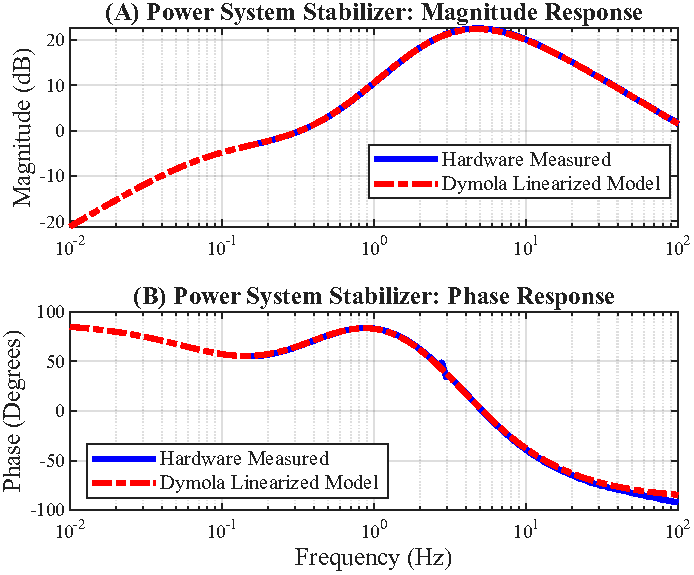
\includegraphics[width=0.9\columnwidth]{./figures/sec06-PSS-bode.pdf}}
    \vspace{-2ex}
    \caption{Frequency response of the \controller{}. Blue: NUCLEO-L476RG running the eFMU, Red: Dymola linearized model.}
    \label{fig:freq-plot-pss}
    \vspace{-2ex}
\end{figure}

First, an open-loop frequency response experiment was conducted on the \controller{}. Figure \ref{fig:freq-plot-pss} shows the Bode plot obtained by analyzing the linear model generated from Dymola (by linearizing the model in Figure \ref{fig:pssvariants}(D)) in a red dashed line, along with the measured Bode plot measured from the hardware (blue line). The excellent agreement of both traces confirms that the \controller{} simulation is running as expected. If the timer's time step on the NUCLEO-L476RG was not configured to exactly match the time step set in Dymola's eFMU export, the entire graph would maintain the same shape but shift horizontally along the frequency axis. 

\begin{figure}[t!]
    \centerline{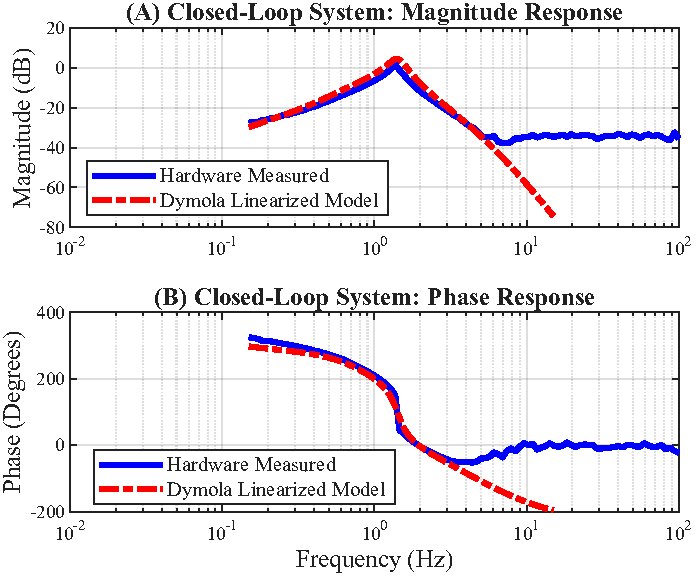
\includegraphics[width=0.9\columnwidth]{./figures/sec06-CLsys-bode.pdf}}
    \vspace{-2ex}
    \caption{Frequency response of the closed-loop test. Blue: hardware measurements, Red: Dymola linearized model.}
    \label{fig:freq-plot-cl}
    \vspace{-2ex}
\end{figure}

The closed-loop experiment was then conducted. Figure \ref{fig:freq-plot-cl} shows the Bode plot obtained by linearizing the model in Figure \ref{fig:closed-loop-simulation} in Dymola, and the one measured during the experiment. Although there is no perfect alignment in this case, they match closely enough to indicate that the eFMU is producing results that are highly consistent with the offline simulation. Measurements at $\approx$5 Hz appear to flatten according to Figure \ref{fig:freq-plot-cl}~(B), albeit with a jagged nature due to noise. This is likely due to the Analog Discovery 3 hitting its measurement noise floor, where it cannot accurately resolve the frequency response at that level of sensitivity anymore, and the limitations of the used onboard ADCs and DACs.

\paragraph{Computation time analyses:} A critical requirement of the CHiL tests is to validate that there are no real-time violations (called overruns), i.e., the \controller{} and \plant{} always finish computing a sampling before a subsequent timer interrupt triggers, requesting the next sampling cycle to be evaluated. To verify this, onboard LED 2 on either board is used (cf. Figure \ref{fig:wiring-diagram}); whenever an overrun is detected, it turns on green for 30 s for the \controller{} or yellow for 5 s for the \plant{}. Note, that LEDs are also used for indicating error signals from the eFMU production codes (like when the embedded linear solver failed due to a singularity). Since the NUCLEO-L476RG of the \controller{} only has LED 2 available for user programs, it is shared for overrun detection and error signals; thus, if it turns on it could be either an overrun or an error signal. For the NUCLEO-H723ZG of the \plant{}, LED 3 (red) is used to indicate error signals.

Although LEDs are helpful for diagnostic purposes, they do not provide any information to which degree real-time requirements are satisfied (if they are); but the headroom for potential additional computations is a good indication if the chosen board is a good fit considering also some security-buffer in case future model changes may cause reasonable additional computational-effort. Therefore, digital GPIO pins were configured to turn on high at the exact start of sampling and to turn off low immediately upon completion (labeled \texttt{D12} in Figure \ref{fig:wiring-diagram} for the \controller{} and \texttt{D2} for the \plant{}). By monitoring the respective pin of either board with the oscilloscope, the true computation time, \texttt{calcTime}, can be physically measured. To be able to plot the computation time relative to the sampling period of that board, timer interrupts are also toggling a separate digital GPIO pin, the \texttt{stepSize} (labeled \texttt{D11} in Figure \ref{fig:wiring-diagram} for the \controller{} and \texttt{D3} for the \plant{}).

\begin{figure}[t!]
    \centerline{\includesvg[width=0.975\columnwidth]{./figures/Fig23.svg}}
    \vspace{-2ex}
    \caption{Computation time (blue) and sampling timer (orange) of the NUCLEO-H723ZG executing the 32-bit floating-point precision eFMI production code (\textit{Release} build) of the \plant{} under (A) steady state, (B) sustained fault injection.}
    \label{fig:calc-time}
    \vspace{-2ex}
\end{figure}

%----------------------------------------------
% Computation time measurements
%----------------------------------------------
% Plant, 32-bit FP, no sustained fault
%   Release build: 96 μs (52% headroom)
%   Debug build: 196 μs (2% headroom)
% Plant, 32-bit FP, with sustained fault
%   Release build: 133 μs (33.5% headroom)
%   Debug build: 239 μs? (19.5% overrun)
% Plant, 64-bit FP, no sustained fault
%   Release build: 146 μs (27% headroom)
%   Debug build: 242 μs (21% overrun)
% Plant, 64-bit FP, with sustained fault
%   Release build: 180 μs (9% headroom)
%   Debug build: 279 μs (39.5% overrun)
%----------------------------------------------

For the \textit{Release} build of the \plant{} the oscilloscope measurements in Figure \ref{fig:calc-time} show that its computation time is well within the 0.2 ms time window between two samplings, with ${\approx}52\%$ headroom in steady state (${\approx}96\mu{}s$ computation time) as shown in (A) and ${\approx}33.5\%$ headroom (${\approx}133\mu{}s$ computation time) during sustained fault as shown in (B). The low-cost NUCLEO-H723ZG with its 550 MHz ARM Cortex-M7 can be used as real-time platform for OpenIPSL power generator simulations.

As can be seen comparing Figure \ref{fig:calc-time}~(A) and (B), there are significant computational differences whether faults are injected or not. The GALEC code of the \plant{} is dominated by a system of linear equations $Ax=b$, with the respective GALEC built-in function call \texttt{solveLinearEquations(A, b)}. If no fault is injected, many elements of the $A$-matrix and $b$-vector become 0, i.e., $A$ and $b$ are sparse. The implementation of \texttt{solveLinearEquations} in the generated production code avoids unnecessary computations in case of 0-elements. As a consequence, computation time drops significantly if no fault is injected. For that reason, our real-time capability validation in Figure \ref{fig:calc-time}~(B) is under sustained fault injection regardless of the \plant{} becoming unstable beyond the point of recovery.

Note that the \textit{Debug} build of the \plant{} overruns in case of sustained fault injection (${\approx}239\mu$ computation time, i.e., ${\approx}19.5\%$ overrun); it is not suited for hard real-time application on the NUCLEO-H723ZG, stressing the requirement for good SiL testing support as demonstrated in Section~\ref{sec:modelica-based-sil-tests} enabling offline debugging in case of functional errors without real-time constraints. For completeness, we also investigated the 64-bit floating-point precision production code of the \plant{}; the \textit{Release} build is only just real-time suited with ${\approx}9\%$ headroom (${\approx}180\mu$ computation time) in case of sustained fault. We consider ${\approx}9\%$ headroom to tight however, to be on the safe side anticipating future minor model changes. Of course, the \textit{Debug} version of the 64-bit floating-point precision \plant{} is out of question with already ${\approx}21\%$ overrun without sustained fault and ${\approx}39.5\%$ overrun with.

For the \controller{}, the \textit{Release} build has ${\approx}92.17\%$ headroom (${\approx}15.67\mu{}s$ computation time), regardless whether faults are injected in the \plant{} or not. In the case of the \controller{}, also the \textit{Debug} build can be deployed with a comfortable headroom of ${\approx}82.83\%$ (${\approx}34.35\mu{}s$ computation time). Ample headroom for the \controller{} is not only beneficial for further, more advanced, stabilizer models, but also crucial in the safety-critical domain, where extensive automatic compiler optimizations like \texttt{-O3} in case of the \textit{Release} build might be considered potentially unsafe for which reason only the \texttt{-O0} non-optimized code of the \textit{Debug} build can be deployed.

\section{Conclusions and future work}\label{sec:conclu}

We presented a MBSE workflow that streamlines power system stabilizer design and deployment on low-cost microcontrollers leveraging the eFMI Standard. By introducing the \texttt{OpenIPSL\_CHIL} library, we established a ``single source of truth'' from physics-based, acausal Modelica models to production C code, clearly separating physics modeling from embedded development. All models, eFMUs, and C projects are provided open-source\footref{fnt:pss-repository} as an extensible workbench framework ultimately empowering researchers to rapidly prototype grid controllers with guaranteed traceability and significantly reduced capital expenditure.

Our systematic MiL, SiL, and CHiL design processes do not only guide development from off-line, continuous simulation models toward safety-critical, hard real-time suited, sampled embedded application, but also enable validation of intermediate designs of the various abstraction levels, significantly reducing the risk of late-stage issues with hard to trace sources of error. Verifying functional correctness via SiL testing provides strong confidence for deployment; once SiL tests pass, HiL system integration mainly involves checking memory fit and real-time execution on the target.

The mostly automatized MBSE process thereby supports iterative development cycles from Modelica models to deployable embedded code, enabling rapid prototyping for target switches and remodeling. The presented plant, for example, had to be redeployed on several targets due to real-time violations and IO pin restrictions before finally settling with the NUCLEO-H723ZG; and likewise the controller design underwent several iterations for signal-noise handling and real-time suited parameter-fitting before CHiL results have been satisfactory. And instead of using the built-in ADCs and DACs of the selected microcontrollers as well as the power supplies provided onboard, we could improve signal-to-noise ratios by using dedicated external ADC and DAC components with careful design without further microcontroller upgrades; such hardware setup redesign would have to be reflected in the model (e.g., filter configurations, parameters, etc), confirming the need of an MBSE-supported iterative development process along the lines of eFMI.

Besides systematic functional testing, we also validated the non-functional quality of the production code generated by the used eFMI tooling. Production code analyses confirm MISRA C:2023 and SEI CERT C Coding Standard\footref{fnt:sei-cert-c} compliance; execution time measurements confirm real-time capability; and the rigorous error signaling of eFMI GALEC confirms the absence of numerical issues.

Last but not least, our approach dramatically reduces capital expenditure. It reduces software licenses to only Dymola (with \textit{Dymola Source Code Generation} option) while using free development tools for the STM32 microcontrollers. And although eFMI was not designed for real-time plant simulation, we show that it has strong potential for that use, eventually replacing proprietary real-time platforms that typically cost $\gg$\$50,000 with $<$\$50 microcontrollers. This came as a surprise to us. Our original plan was to use one of the established real-time platforms, like from dSPACE, for the power generator plant-model (and only deploy the PSS controller-model on a microcontroller); we only tried eFMI-based deployment of the plant-model out of curiosity how far we can get with Dymola's eFMI tooling, but soon figured this may indeed work out!

Future research will concentrate on both the modeling and eFMU integration sides. We intend to work on scaling our current proof-of-concept to cover a broader spectrum of PSS models, and on creating templates that support a variety of embedded hardware boards from the STM32 family. An important objective is to exploit the eFMI recalibration to enable online parameter tuning, thereby allowing the PSS to adapt its behavior to real-time grid conditions. Finally, we plan to showcase the integration of eFMUs (exported as source code FMUs or the eFMI production code directly system integrated) into industrial real-time platforms from dSPACE, Typhoon HIL, and OPAL-RT Technologies.

\section*{Acknowledgment}

The authors would like to thank:

\squishlist
    \item Fabio Ballari and the CATIA\regtm{} Champions program at Dassault Systèmes\regtm{} for providing complimentary access to the \textbf{3D}EXPERIENCE\regtm{} platform\footnote{\tiny{\url{https://www.3ds.com/3dexperience/}}} and its Systems Software Production Engineer (SOP-OC) capabilities, which enabled the early development of this work.
    \item Dr. Christopher R. Laughman at Mitsubishi Electric\regtm{} Research Laboratories for an unrestricted gift grant to Rensselaer Polytechnic Institute\regtm{} that funded the embedded hardware behind this project.
    \item Daniel Marjamäki and Magnus Janagård of Cppcheck Solutions AB\footref{fnt:cppcheck-premium} for providing a free license of Cppcheck Premium.
\squishend

\section*{Appendix: Related work}

Previous research has transitioned advanced controllers to real-time platforms, such as National Instruments hardware-based wide-area controllers in \cite{Vanfretti2018_Audur}, \cite{epri} and \cite{Schoenwald2017}. Moreover, recent industrial trials by Red Eléctrica and RTE on HVDC interconnectors \cite{Renedo2023} demonstrate that aligning simulation models with actual hardware behavior is now paramount. 

Industrial platforms like GE's PhasorController \cite{Golshani2021} utilize deterministic PLC engines for real-time grid control; however, these solutions typically rely on manual imperative programming rather than the automated code synthesis central to a formal MBSE workflow, which severs the traceability between the physical model and the target implementation. The limitations of manual coding are particularly acute in enabling modern adaptive control strategies; for example, recent Terna research proposes online PSS tuning based on estimation \cite{Lauria2024_SEGAN}, while our previous work demonstrates the need for a continuous controller redesign \cite{Bombois2024, Vanfretti2024_IFAC}.

This lack of traceability is similarly evident in the field of power system simulation, where the exchange of models within industry remains limited. The IEEE/CIGRE DLLs Guideline (ICDMS) \cite{CIGRE958} attempts to address model sharing by distributing vendor algorithms as precompiled DLLs; nevertheless, these remain 'black boxes' containing likely hand-written code, continuing to sever the connection to the underlying physics. As such DLLs are not suitable for real-time simulation, CHiL testing remains limited. This is even more challenging when trying to migrate large-scale models, such as the Continental Europe model, to real-time targets, which remains problematic \cite{Ramirez2024}. However, recent work has championed Modelica and FMI~\cite{FMIv2:0:2} to solve this, enabling models from the Open-Instance Power Systems Library (OpenIPSL) to be executed directly on dSPACE hardware \cite{deCastro2023_RealTime}.

In this context, the eFMI Standard \cite{eFMI_Standard, Lenord2021} enables a continuum from offline simulation into the domain of hard real-time and safety-critical embedded software. Unlike opaque DLLs, eFMI guarantees traceability via GALEC, ensuring that production code is systematically generated from a source physics model. Although proven in automotive applications \cite{Ultsch2021, Kamp2025, Armugham2021}, its application in power system control is first explored in this paper.

\printbibliography
%\newpage
%\section*{Annex}

\end{document}
